% ============================================================
%  ANEXO IX - DISENO CENTRADO EN EL USUARIO
%  DocumentChain - Sistema de Gestion Documental con Blockchain
% ============================================================
\documentclass[11pt, a4paper]{article}
\usepackage{fontspec}
\usepackage[spanish]{babel}
\usepackage{graphicx}
\usepackage{float}
\usepackage{xcolor}
\usepackage{booktabs}
\usepackage{enumitem}
\usepackage[
    colorlinks = true,
    linkcolor  = black,
    urlcolor   = black,
    citecolor  = black
]{hyperref}
\usepackage{geometry}
\geometry{left=2.5cm, right=2.5cm, top=3cm, bottom=2.5cm, headheight=55pt, headsep=0.8cm}
\usepackage{fancyhdr}
\pagestyle{fancy}
\fancyhf{}
\lhead{
\includegraphics[height=1.25cm]{USAL-Logo-3820702873.png}}
\rhead{\shortstack[r]{\fontsize{10}{12}\selectfont\textbf{Anexo IX}\\[-1pt]\fontsize{10}{12}\selectfont Diseno Centrado en el Usuario}}
\renewcommand{\headrulewidth}{0pt}
\renewcommand{\footrulewidth}{0pt}
\cfoot{%
    \color{gray}\rule[0.5ex]{0.4\textwidth}{0.8pt}%
    \hspace{0.5cm}%
    \textcolor{black}{\textbf{\thepage}}%
    \hspace{0.5cm}%
    \color{gray}\rule[0.5ex]{0.4\textwidth}{0.8pt}%
}
\newcommand{\autorUno}{David Pérez Velasco}
\newcommand{\tutorUno}{Gabriel Villarrubia González}
\newcommand{\tutorDos}{Sergio García González}
\newcommand{\asignatura}{Trabajo de Fin de Grado}
\begin{document}

\begin{titlepage}
    \centering
    \vspace*{1.5cm}
    {\scshape\LARGE Universidad de Salamanca \par}
    \vspace{1cm}
    {\scshape\Large Grado en Ingenieria Informatica \par}
    \vspace{1.5cm}
    {\huge\bfseries ANEXO IX \par}
    \vspace{0.5cm}
    {\Large\bfseries Diseno Centrado en el Usuario \par}
    \vspace{0.3cm}
    {\large\itshape Sistema de Gestion Documental mediante Blockchain \par}
    \vspace{1.8cm}
    
\includegraphics[width=0.28\textwidth]{USAL-Logo-3820702873.png}

    \vspace{2.2cm}

    {\Large\itshape \autorUno \par}
    \vspace{1.5cm}
    {\large Tutores: \par}
    \vspace{0.3cm}
    {\large \tutorUno \par}
    \vspace{0.2cm}
    {\large \tutorDos \par}

    \vspace{2cm}
    {\large Julio 2026}
    \vspace{0.5cm}

    \asignatura
    \vspace{1cm}
\end{titlepage}

\setcounter{page}{2}
\pagestyle{fancy}
\tableofcontents
\newpage

\section{Introduccion}

Este anexo recoge la metodolog\'ia de dise\~no centrado en el usuario que se ha seguido durante el desarrollo de DocumentChain. El objetivo era asegurar que la soluci\'on, a pesar de apoyarse en tecnolog\'ias complejas como blockchain o IPFS, resultase intuitiva para cualquier persona. Para ello se aplicaron t\'ecnicas de identificaci\'on de necesidades, prototipado, pruebas de usabilidad e iteraciones de mejora.

\section{Identificacion de necesidades}

En este apartado se documentan las tecnicas de necesidad aplicadas para comprender las expectativas de los usuarios finales del sistema.

\subsection{Needfinding}

Para entender qu\'e esperar\'ian los usuarios de un sistema como DocumentChain, el autor parti\'o del an\'alisis del estado del arte y de su propia experiencia en el \'ambito de la gesti\'on documental. De ese proceso surgieron las siguientes necesidades cr\'iticas:

\begin{itemize}
    \item \textbf{Necesidad de autenticidad}: poder garantizar que un documento no ha sido alterado desde que se cre\'o.
    \item \textbf{Trazabilidad}: contar con un historial inmutable de todo lo que ha ocurrido sobre cada documento.
    \item \textbf{Control de acceso}: compartir documentos con permisos granulares, decidiendo qui\'en puede leer y qui\'en puede editar.
    \item \textbf{Firma digital}: disponer de un mecanismo de firma criptogr\'aficamente verificable, sin depender de terceros.
    \item \textbf{Interfaz intuitiva}: que el sistema se pueda usar sin tener nociones de blockchain, wallets ni IPFS.
\end{itemize}

\subsection{Elevator Pitch}

A partir de las necesidades detectadas, se formul\'o la siguiente propuesta de valor, que sirvi\'o como gu\'ia durante todo el desarrollo:

``DocumentChain es una plataforma web que permite gestionar documentos digitales con total garantia de autenticidad mediante blockchain. Cualquier usuario puede subir, compartir, firmar y verificar documentos sin necesidad de conocimientos tecnicos, asegurando que nadie pueda alterar su contenido sin dejar rastro.''

\section{Arquetipos de usuarios}

A continuacion se presentan los arquetipos de usuarios identificados durante la fase de analisis, elaborados a partir de las necesidades detectadas en la etapa de necesidad.

\begin{table}[H]
\centering
\renewcommand{\arraystretch}{1.4}
\small
\begin{tabular}{|l|p{4cm}|p{4cm}|p{4cm}|}
\hline
\textbf{Arquetipo} & \textbf{Perfil} & \textbf{Objetivos} & \textbf{Frustraciones} \\
\hline
Profesional legal & Abogado, notario & Firmar contratos, verificar autenticidad & Procesos manuales, falta de trazabilidad \\
\hline
Administrador TI & Responsable de sistemas & Gestionar usuarios, controlar accesos & Herramientas complejas, falta de auditoria \\
\hline
Usuario general & Cualquier persona & Almacenar y compartir documentos & No entiende blockchain, necesita simplicidad \\
\hline
\end{tabular}
\caption{Arquetipos de usuarios}
\label{tab:arquetipos}
\end{table}

\section{Prototipos y mockups}

\subsection{Prototipado en papel y mockups digitales}

Como paso previo al diseno digital, se realizo una sesion de prototipado en papel con las pantallas principales del sistema (registro, inicio de sesion, listado de documentos y panel de administracion). Esta tecnica permitio iterar rapidamente sobre la disposicion de los elementos antes de invertir tiempo en mockups digitales, reduciendo el numero de correcciones necesarias en fases posteriores.

Posteriormente, se elaboraron prototipos HTML de baja fidelidad para las pantallas principales del sistema. Estos prototipos, disponibles en el directorio \texttt{bocetos-anexo2/minihtml/} del repositorio, permiten visualizar la arquitectura de la informacion y los flujos de navegacion antes de la implementacion final. Las Figuras~\ref{fig:mockup-login} a~\ref{fig:mockup-settings} muestran una seleccion representativa de estos prototipos, comparados con las capturas de la interfaz final.

\begin{figure}[H]
    \centering
    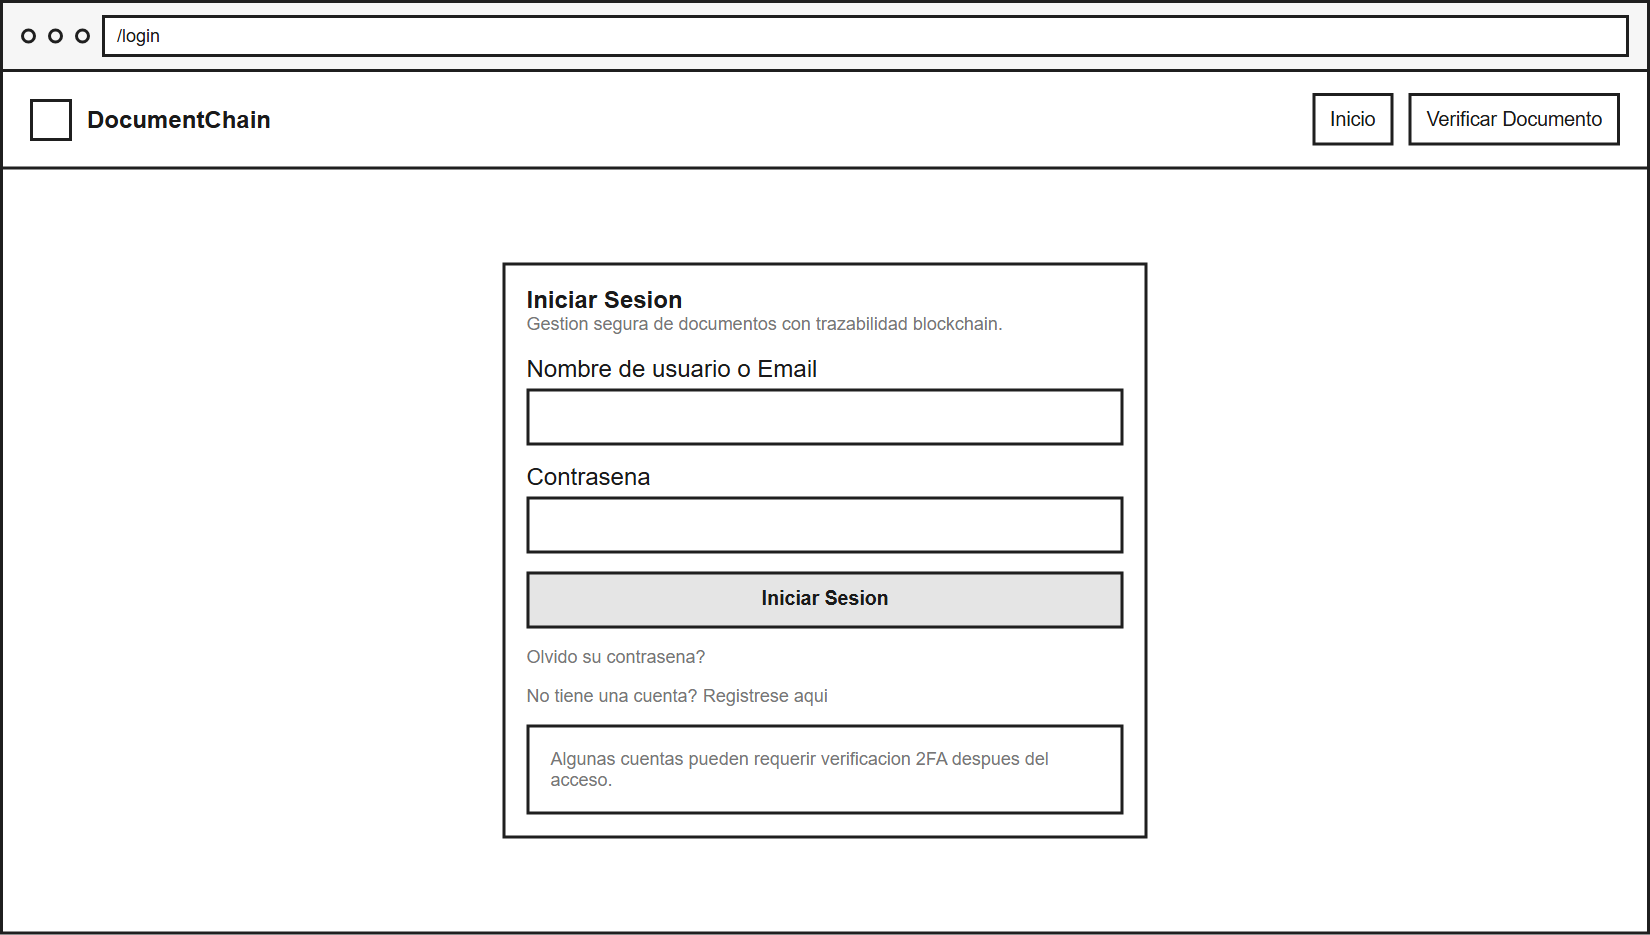
\includegraphics[width=0.45\textwidth]{bocetos-anexo2/login-wireframe.png}
    \hfill
    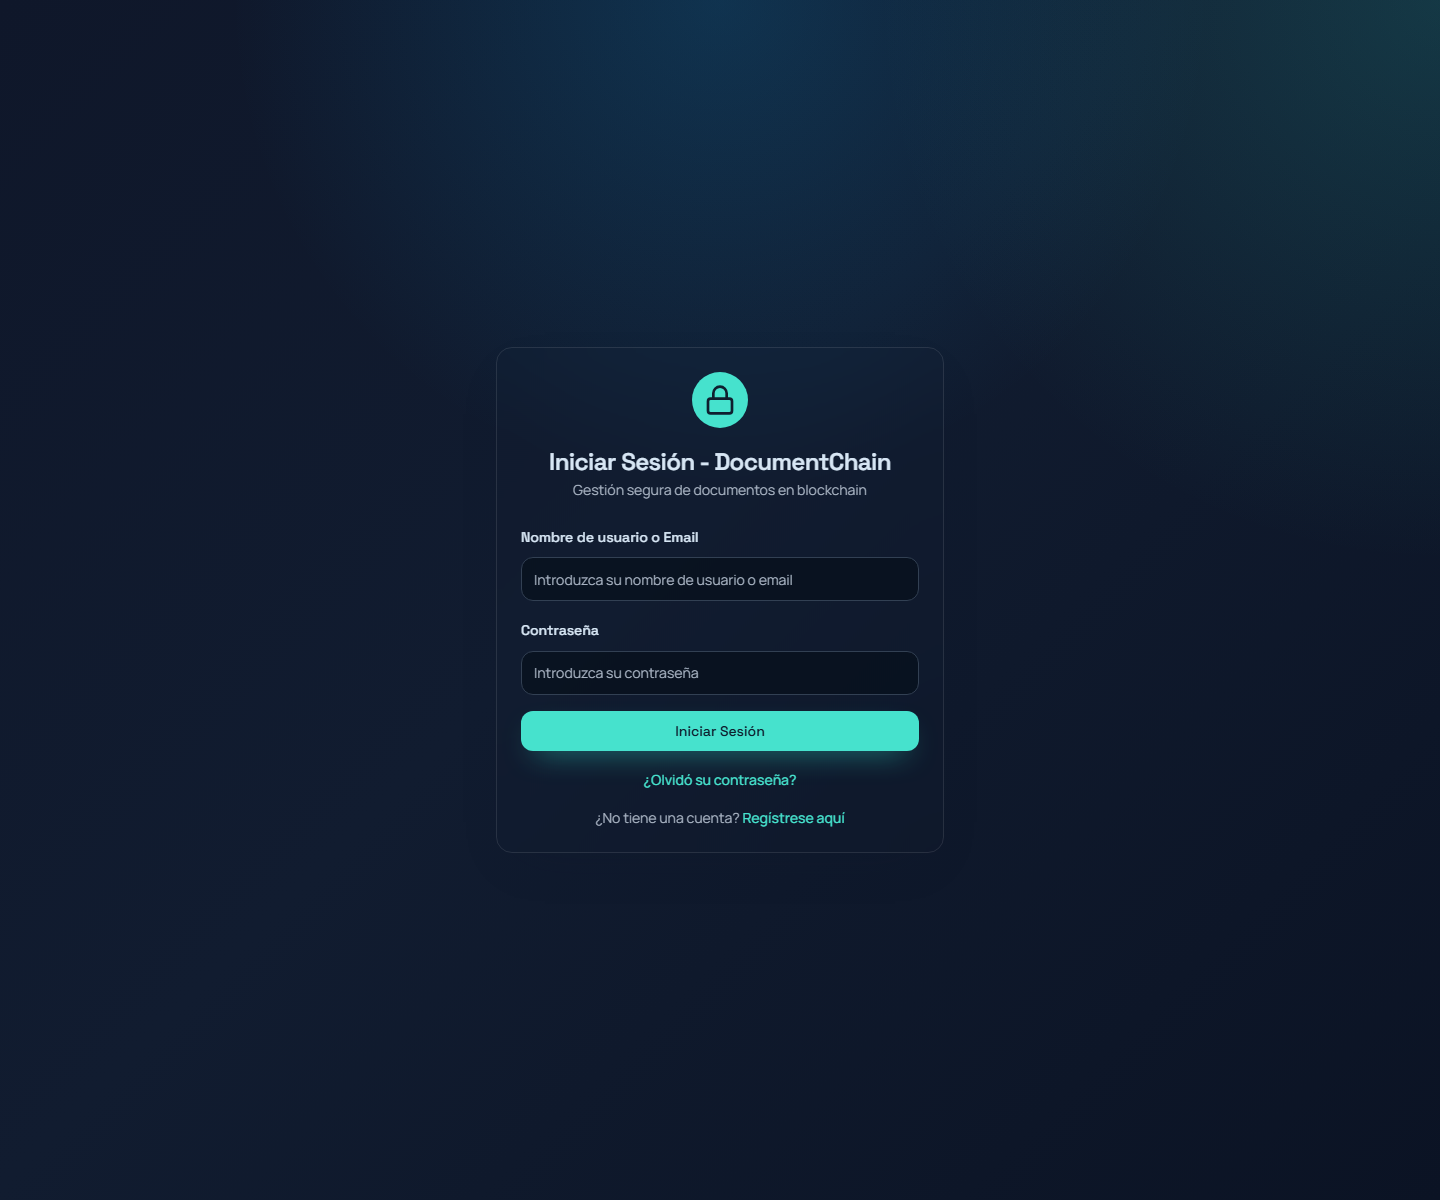
\includegraphics[width=0.45\textwidth]{capturas-ui/login-page.png}
    \caption{Prototipo HTML (izquierda) e interfaz final (derecha) de la pantalla de inicio de sesion}
    \label{fig:mockup-login}
\end{figure}

\begin{figure}[H]
    \centering
    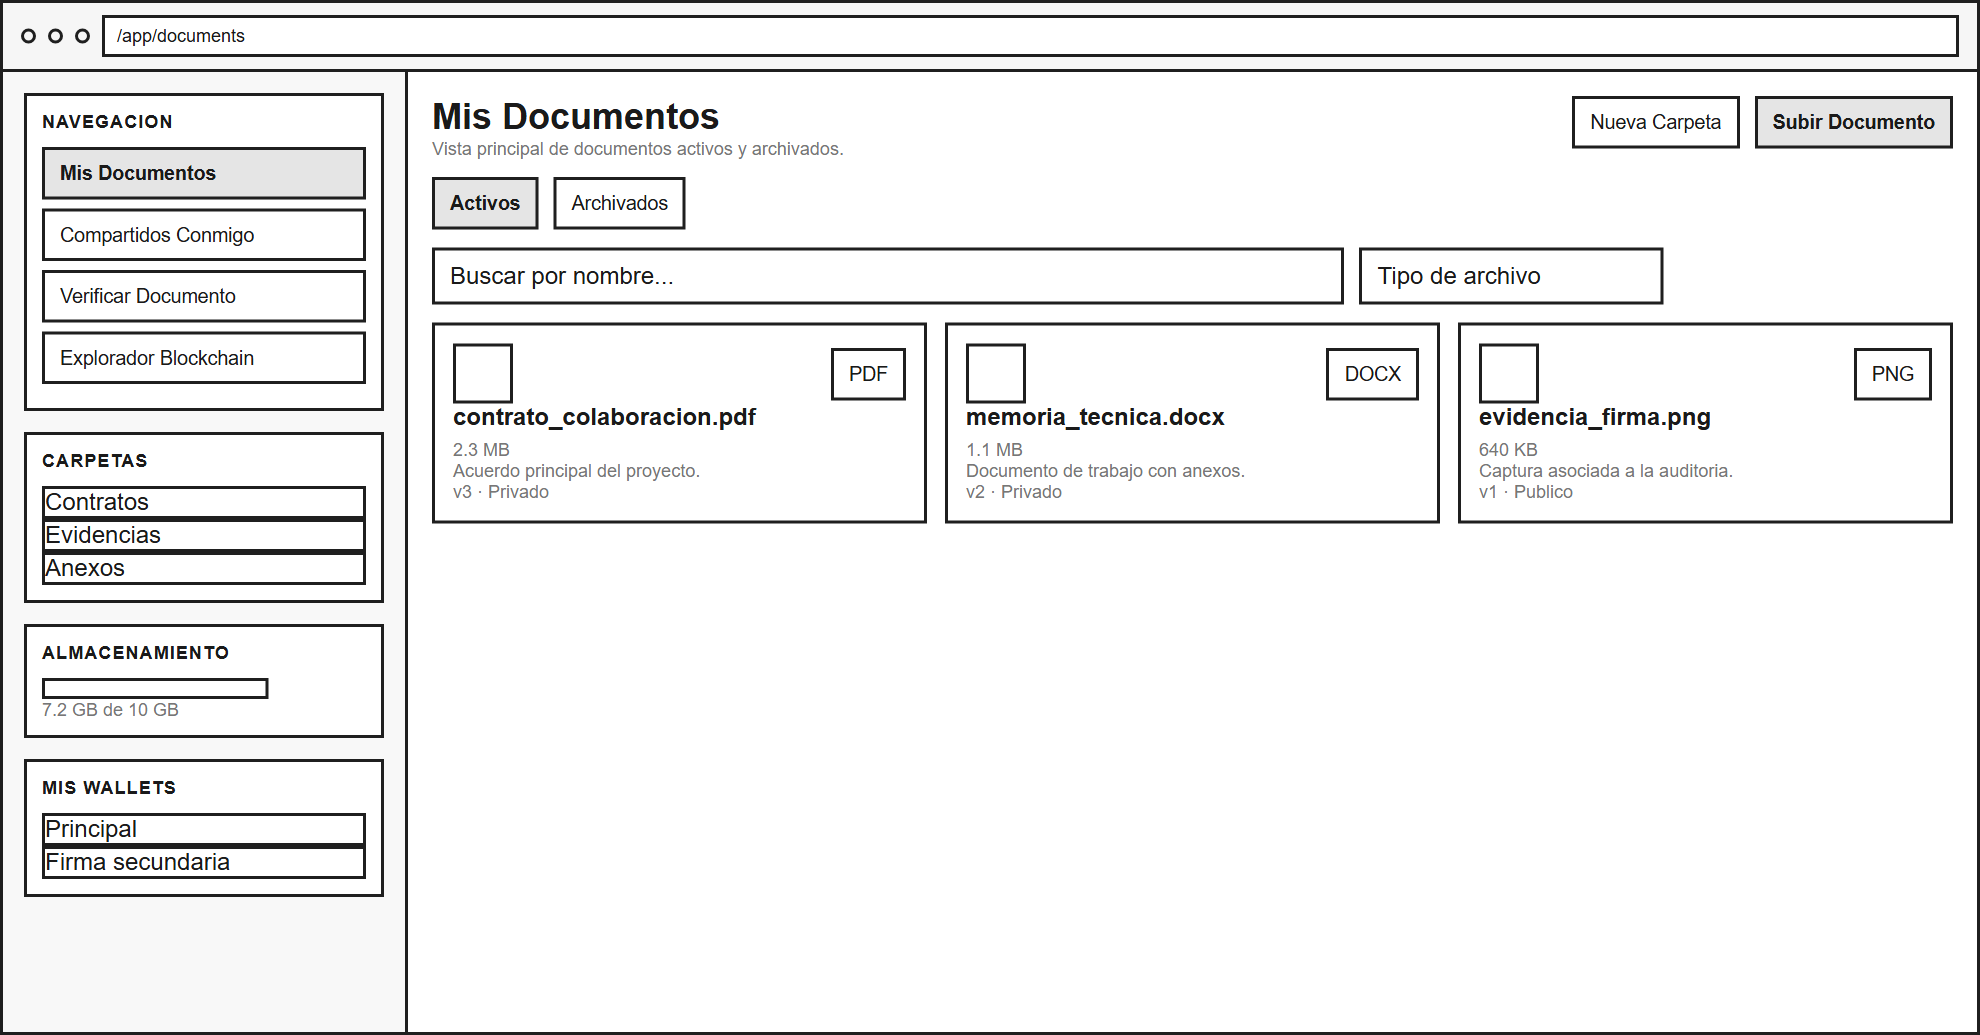
\includegraphics[width=0.45\textwidth]{bocetos-anexo2/documents-dashboard-wireframe.png}
    \hfill
    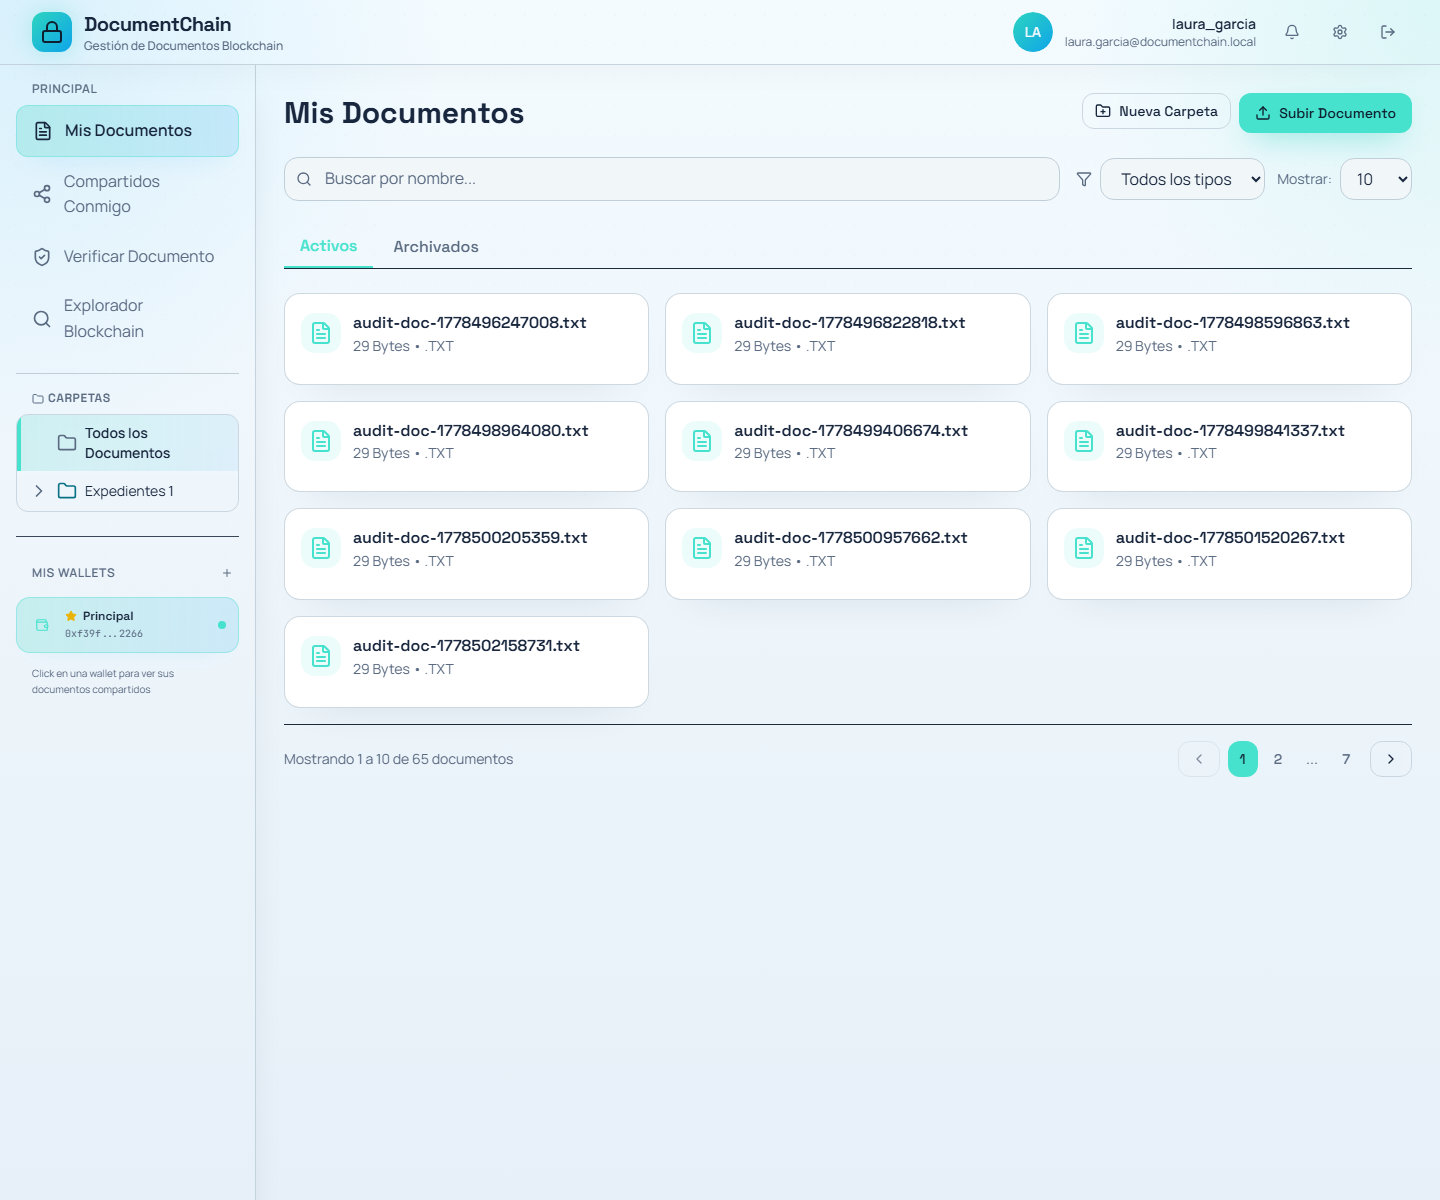
\includegraphics[width=0.45\textwidth]{capturas-ui/documents-page.png}
    \caption{Prototipo HTML (izquierda) e interfaz final (derecha) de la vista principal de documentos}
    \label{fig:mockup-docs}
\end{figure}

\begin{figure}[H]
    \centering
    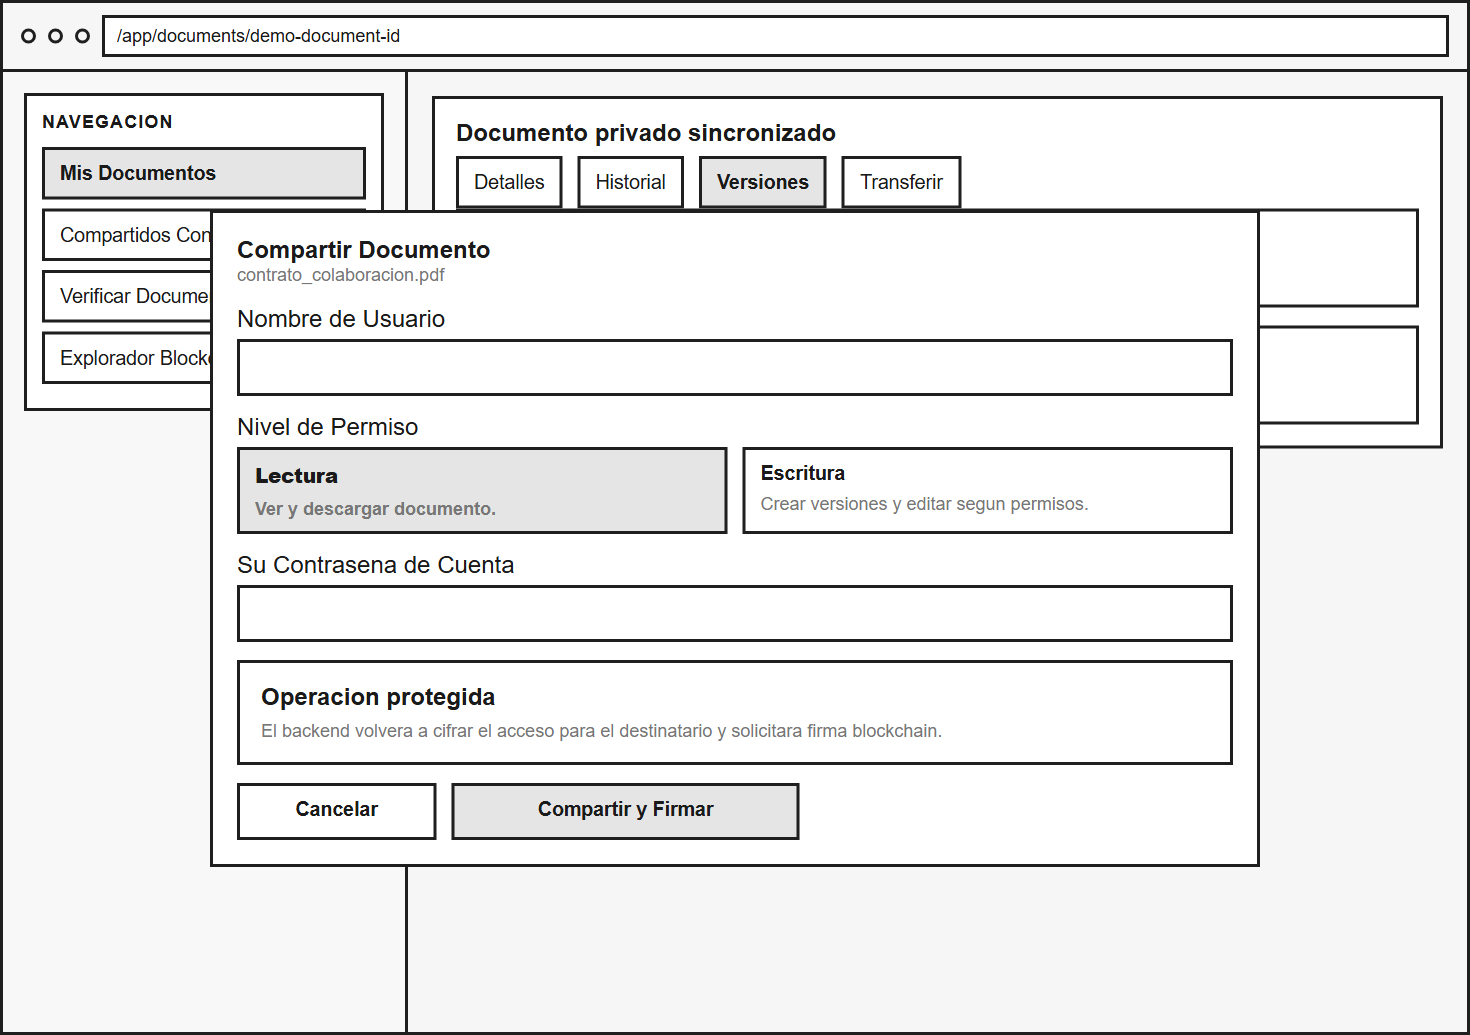
\includegraphics[width=0.45\textwidth]{bocetos-anexo2/share-modal-wireframe.png}
    \hfill
    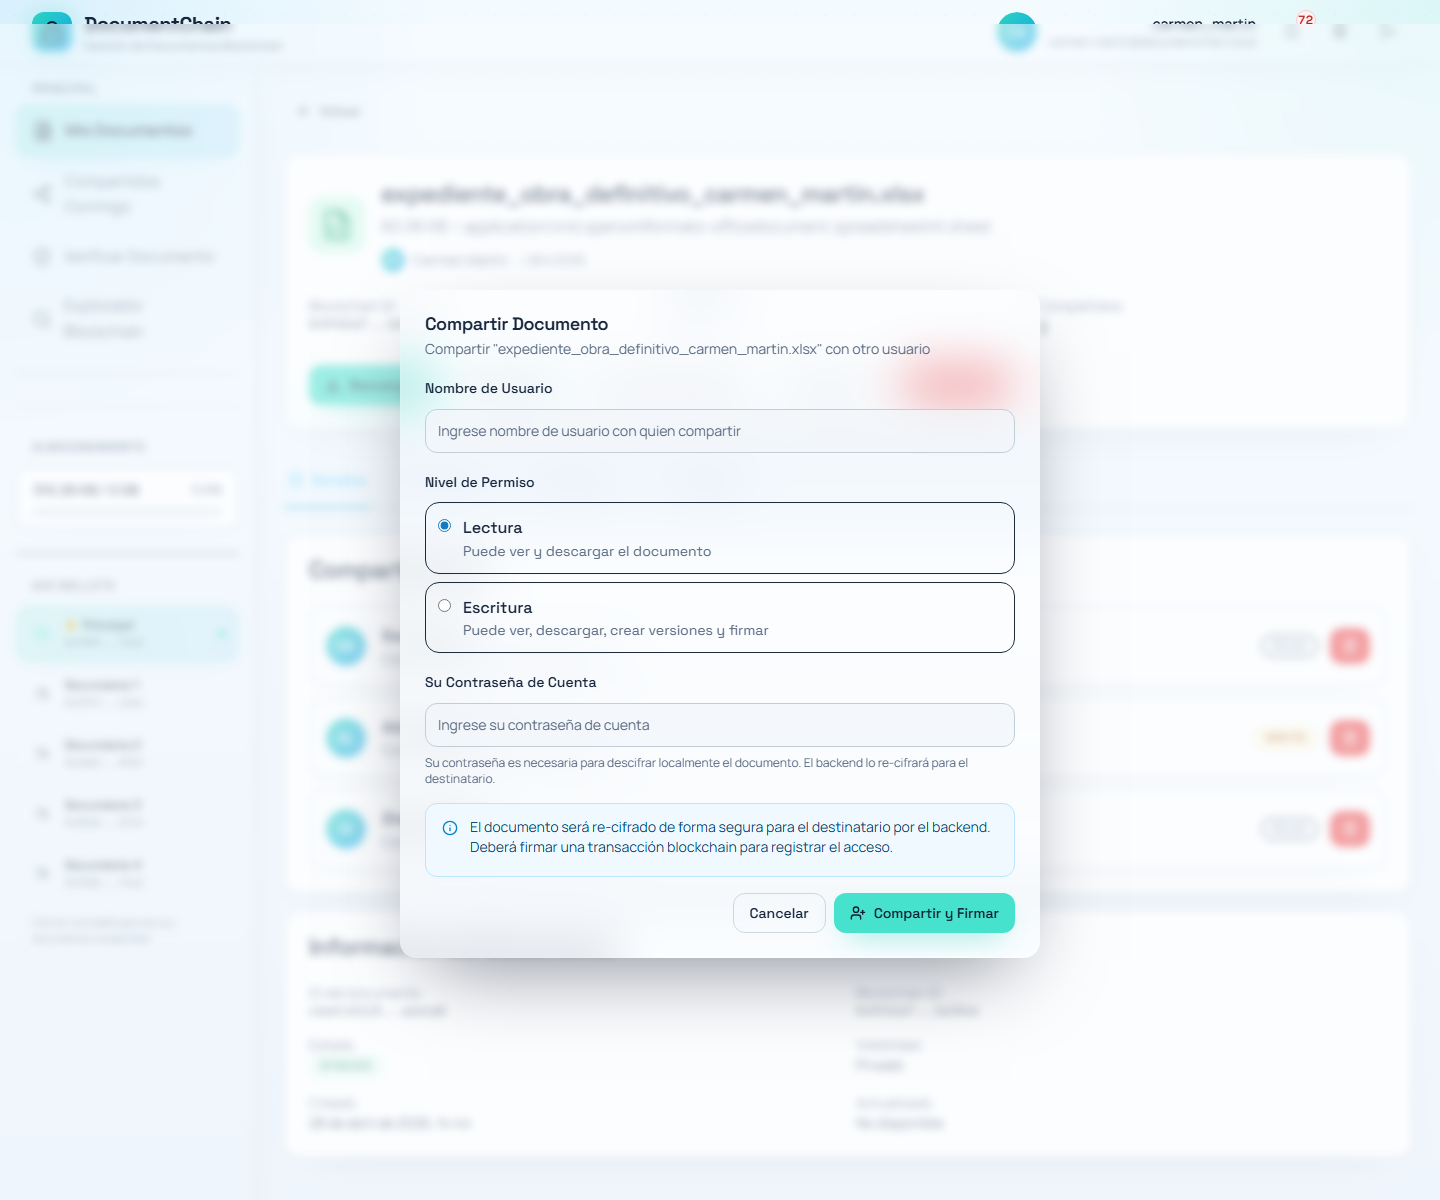
\includegraphics[width=0.45\textwidth]{capturas-ui/share-modal.png}
    \caption{Prototipo HTML (izquierda) e interfaz final (derecha) del modal de compartir documento}
    \label{fig:mockup-share}
\end{figure}

\begin{figure}[H]
    \centering
    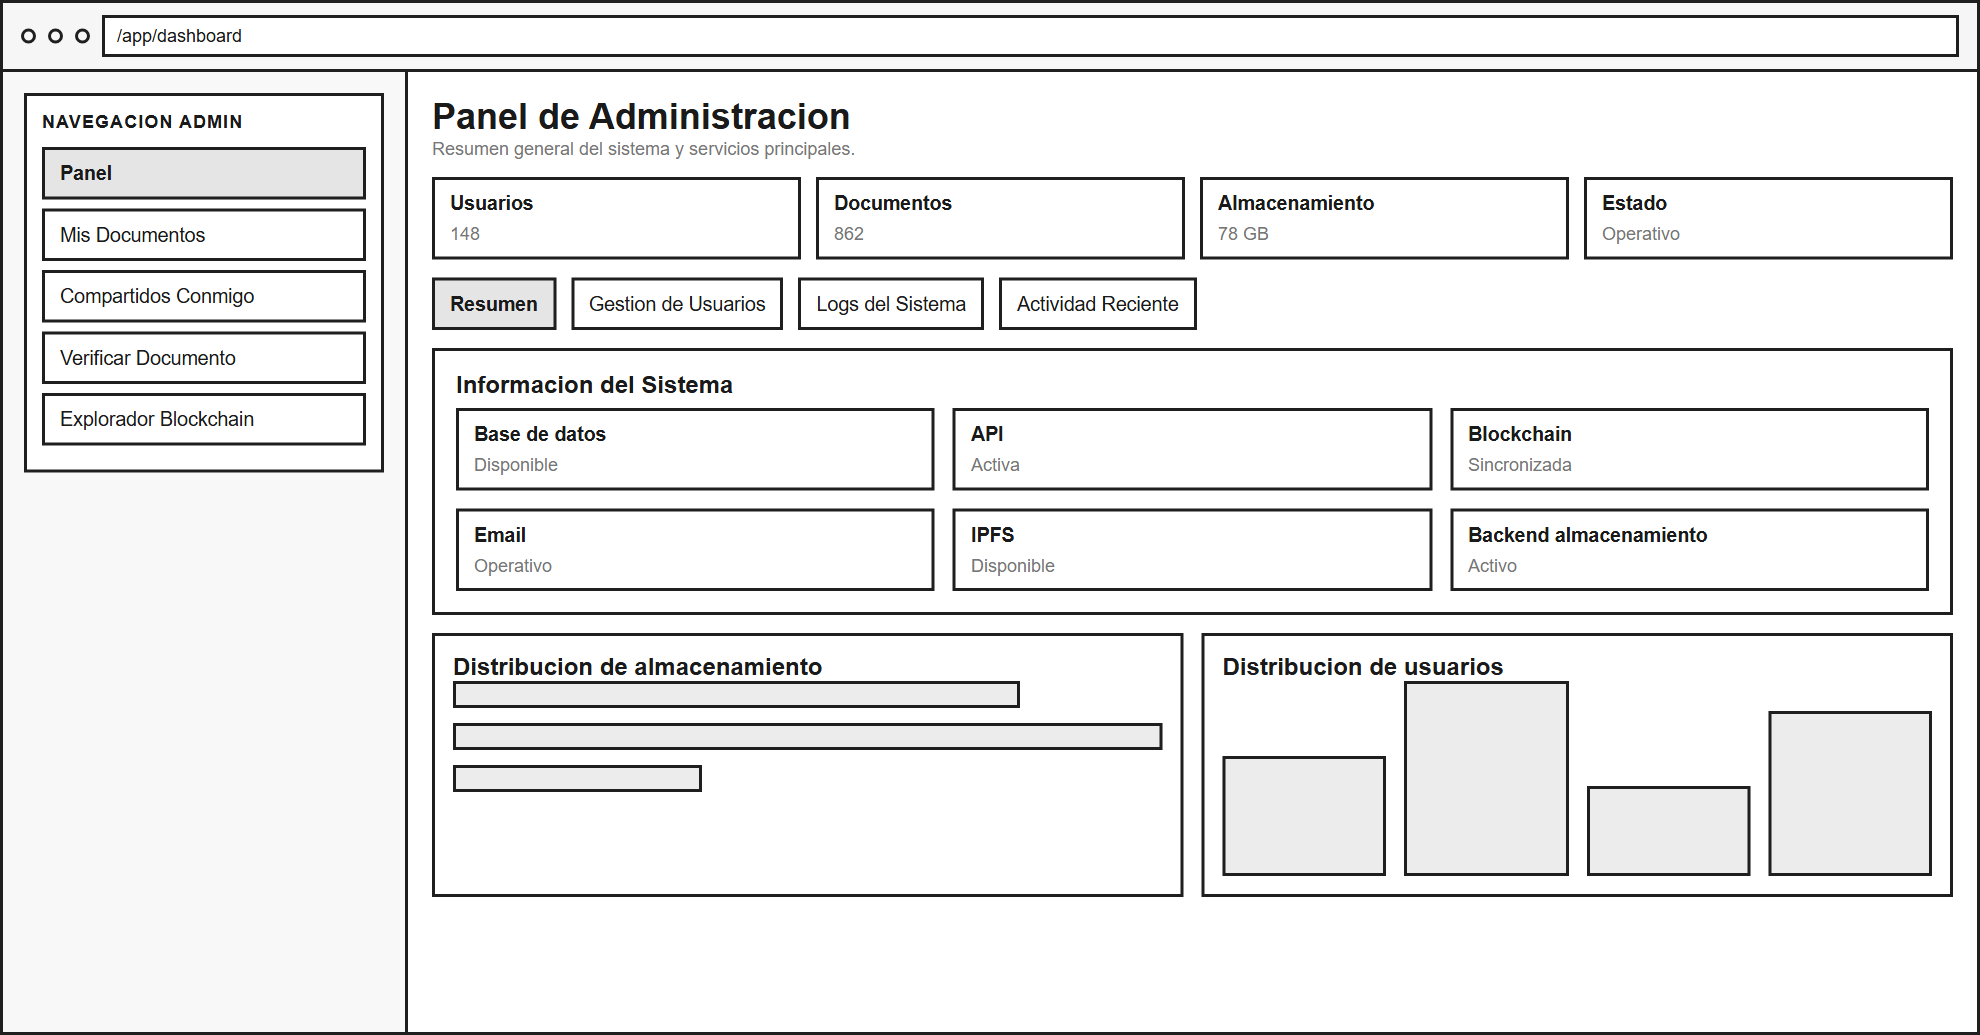
\includegraphics[width=0.45\textwidth]{bocetos-anexo2/admin-dashboard-wireframe.png}
    \hfill
    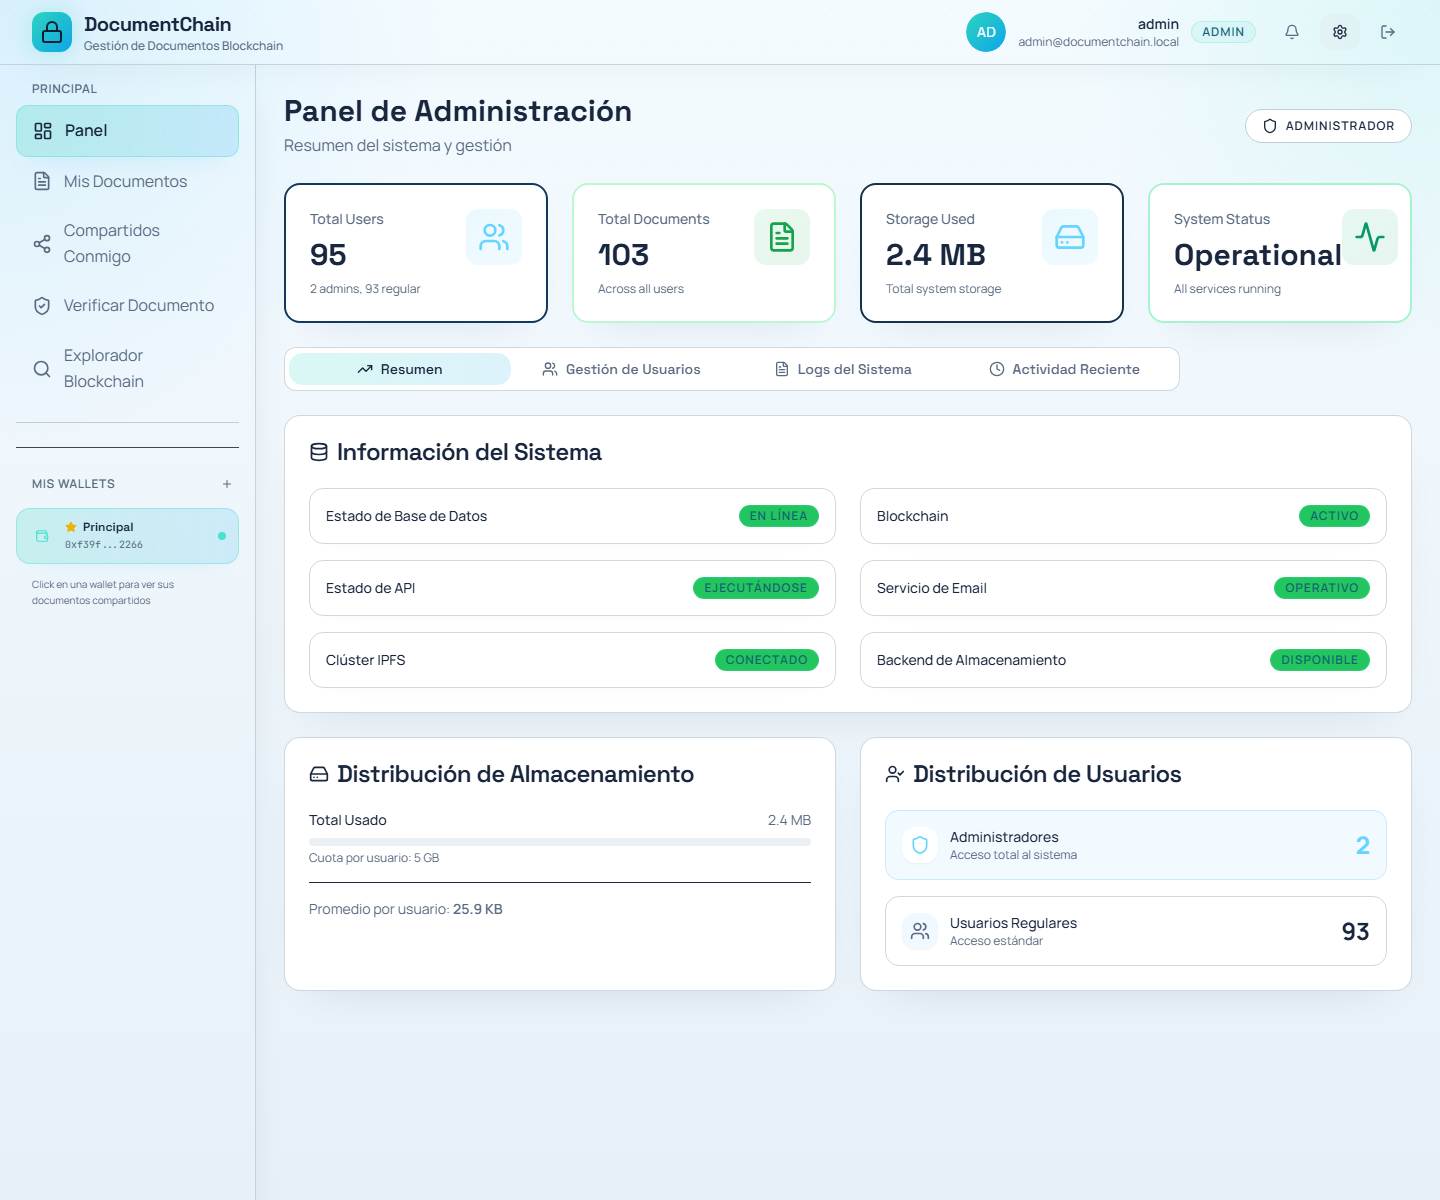
\includegraphics[width=0.45\textwidth]{capturas-ui/admin-dashboard.png}
    \caption{Prototipo HTML (izquierda) e interfaz final (derecha) del panel de administracion}
    \label{fig:mockup-admin}
\end{figure}

\begin{figure}[H]
    \centering
    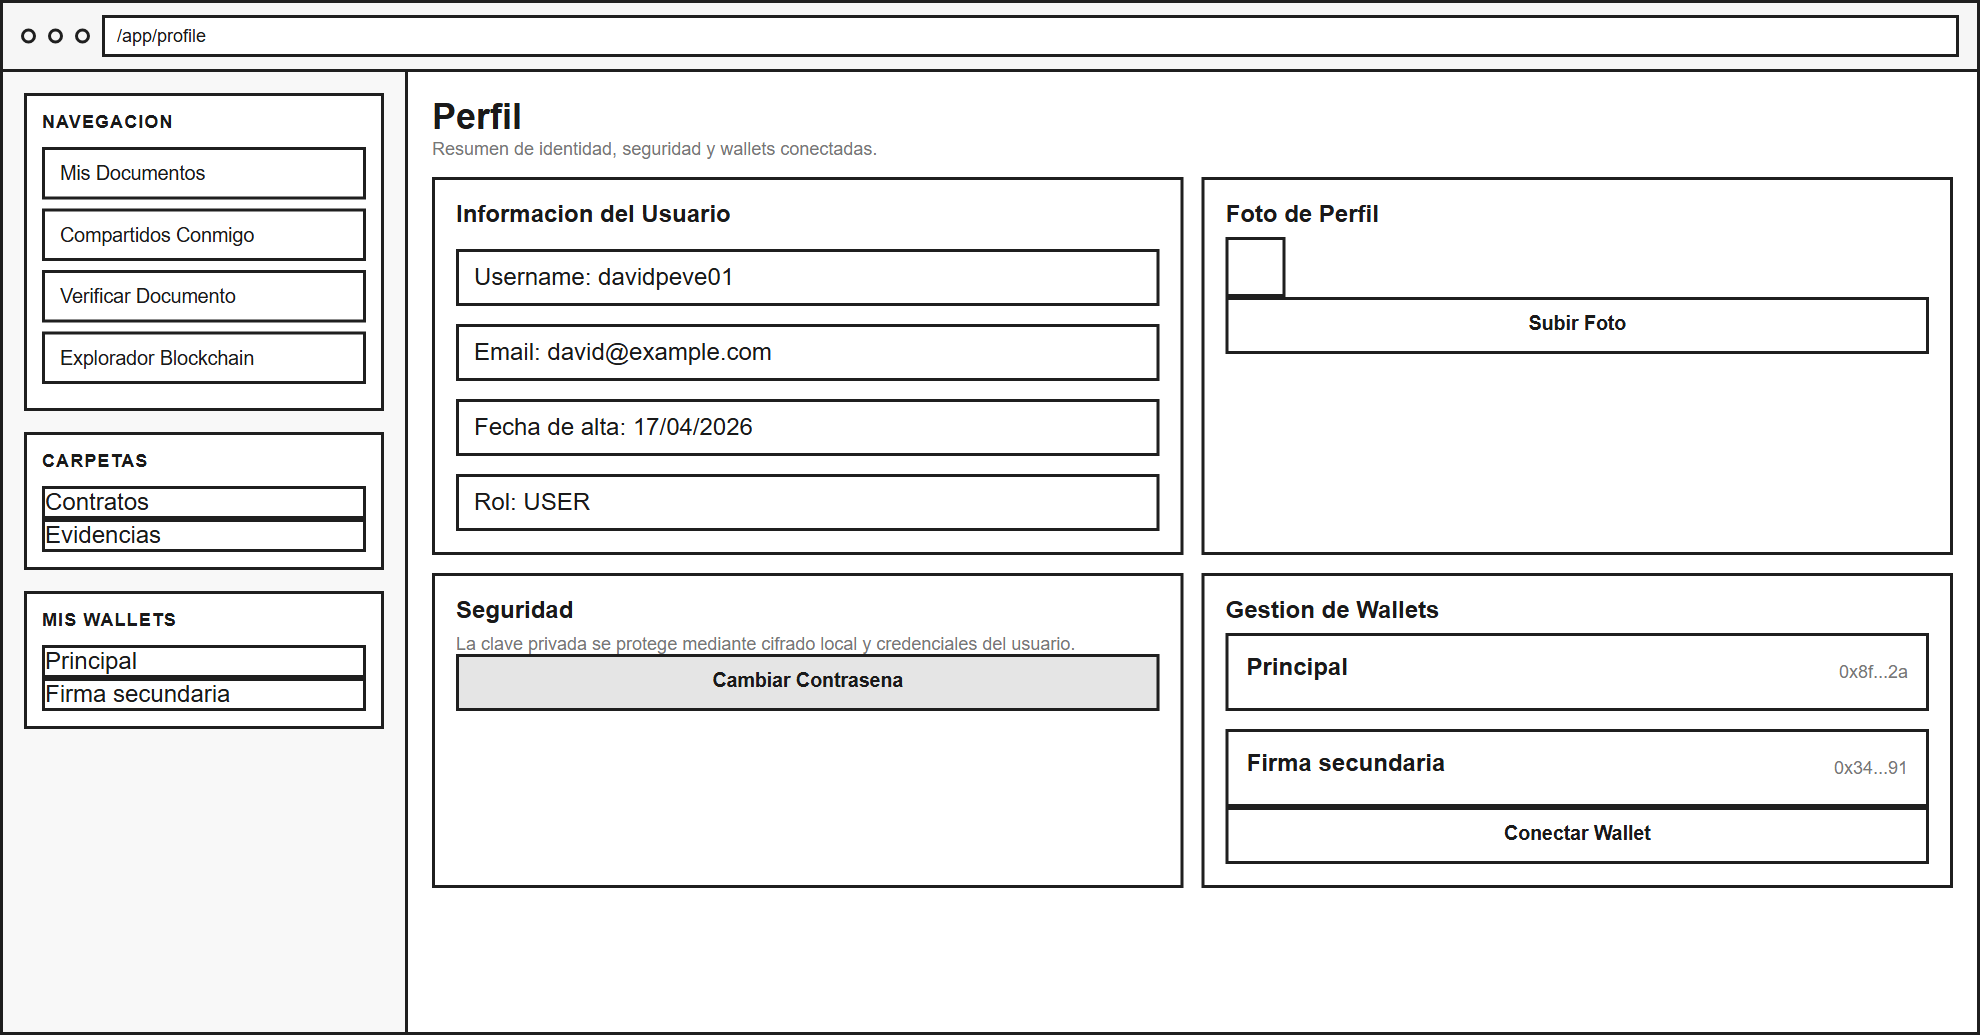
\includegraphics[width=0.45\textwidth]{bocetos-anexo2/profile-wireframe.png}
    \hfill
    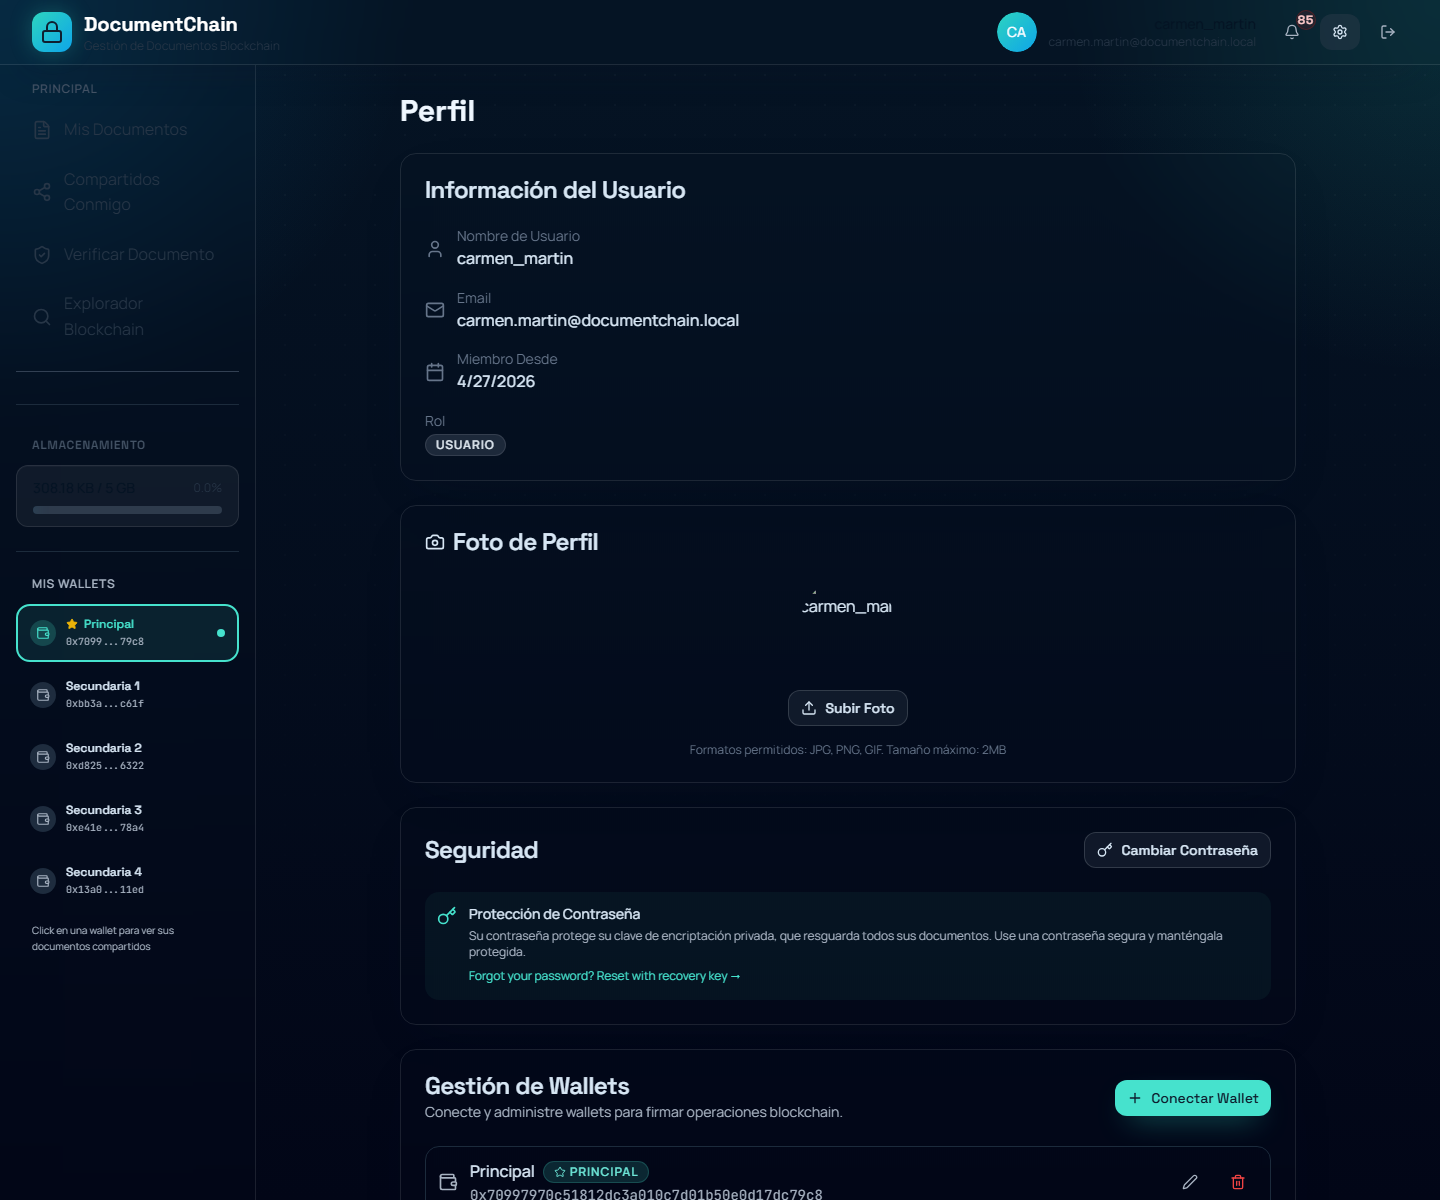
\includegraphics[width=0.45\textwidth]{capturas-ui/profile-page.png}
    \caption{Prototipo HTML (izquierda) e interfaz final (derecha) de la pagina de perfil de usuario}
    \label{fig:mockup-profile}
\end{figure}

\begin{figure}[H]
    \centering
    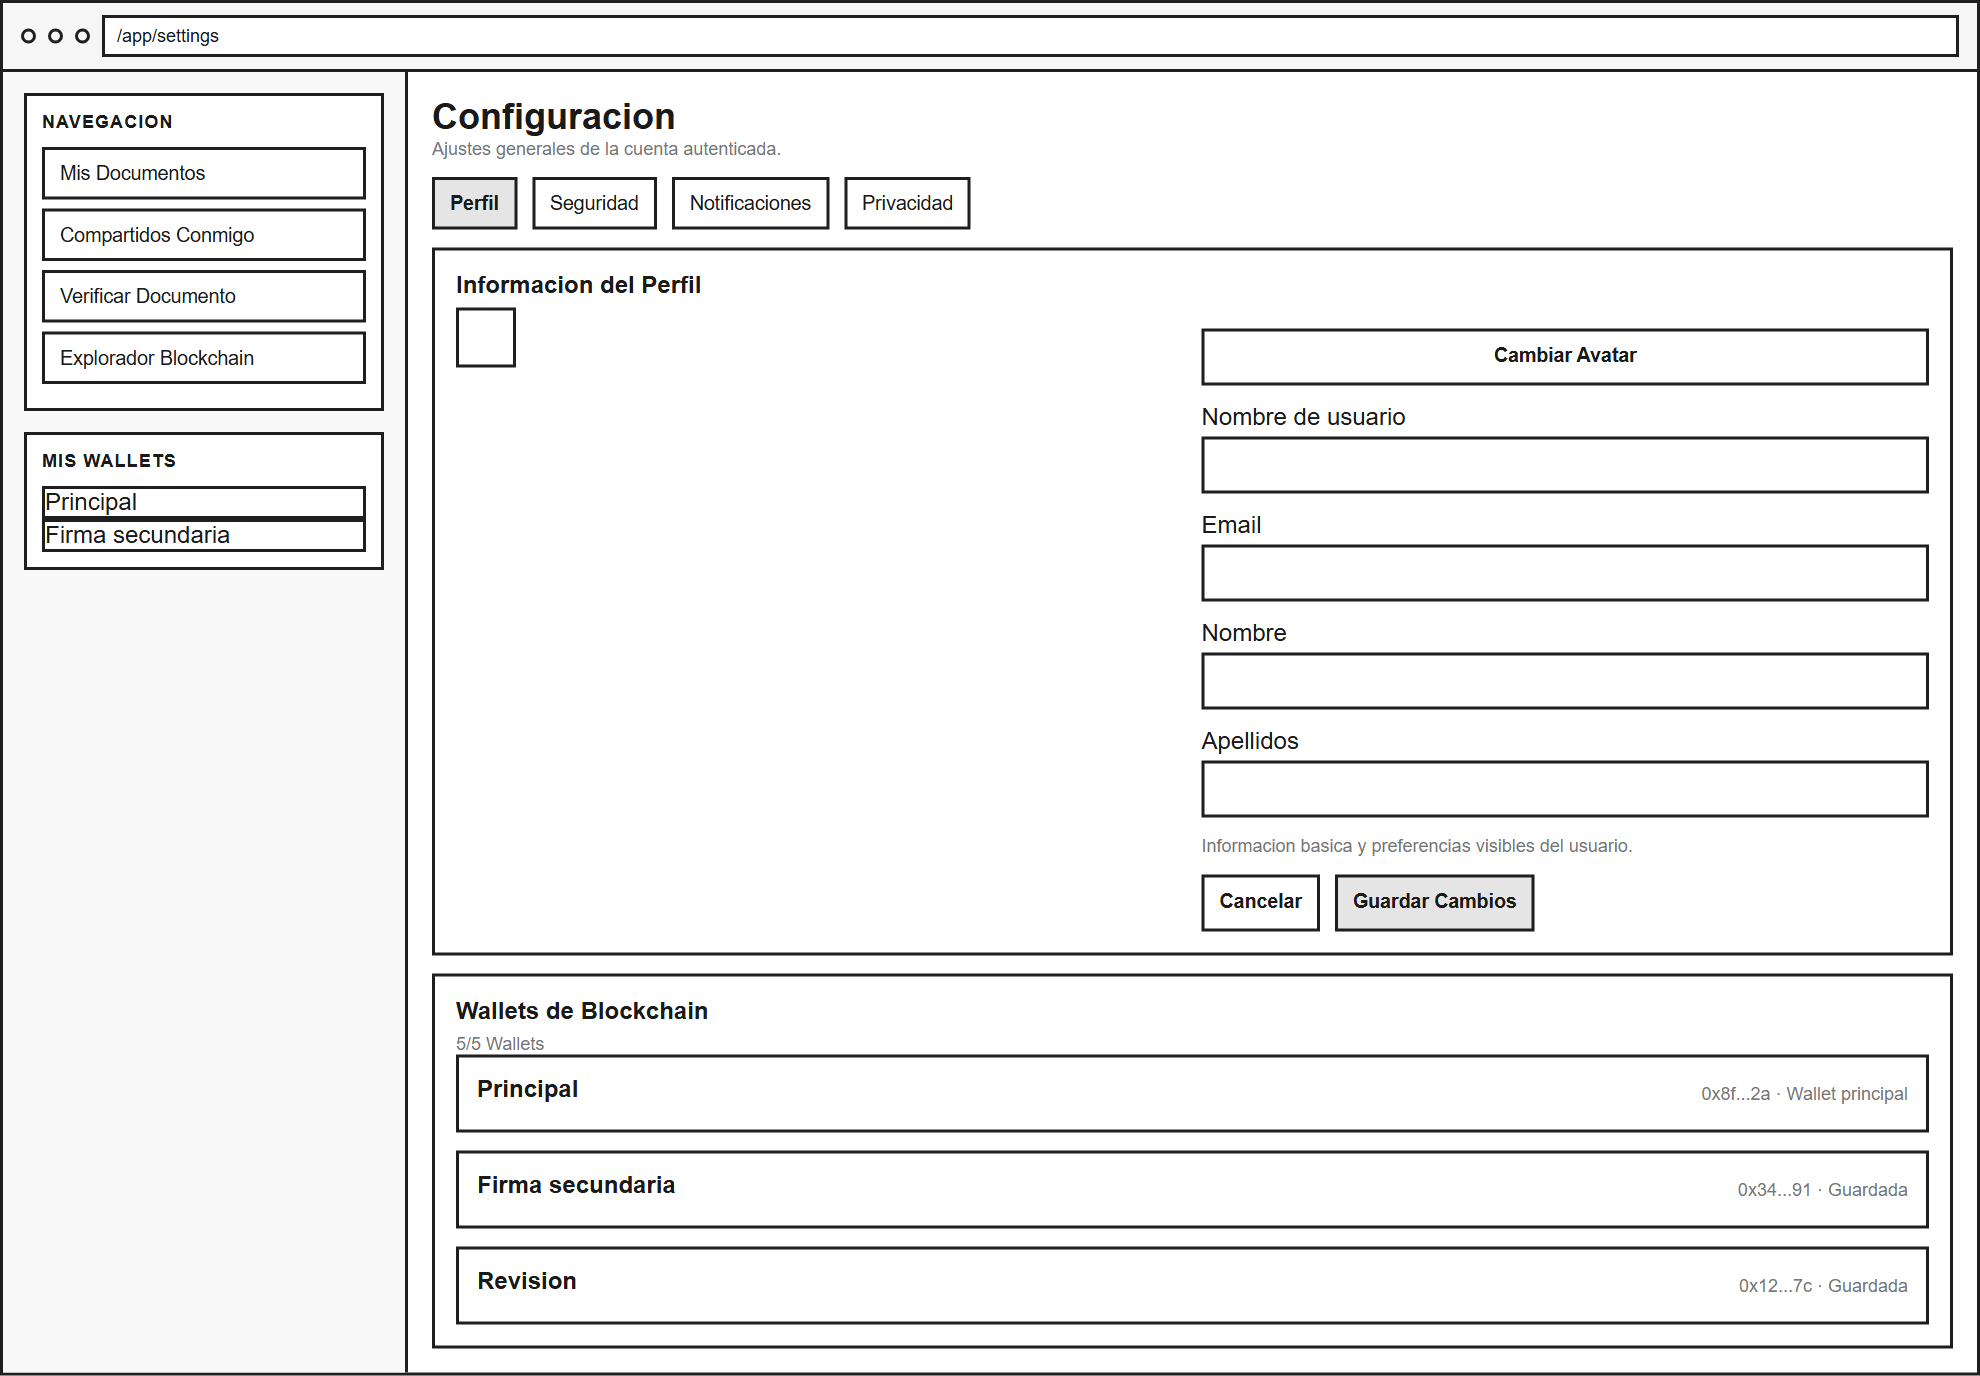
\includegraphics[width=0.45\textwidth]{bocetos-anexo2/settings-wireframe.png}
    \hfill
    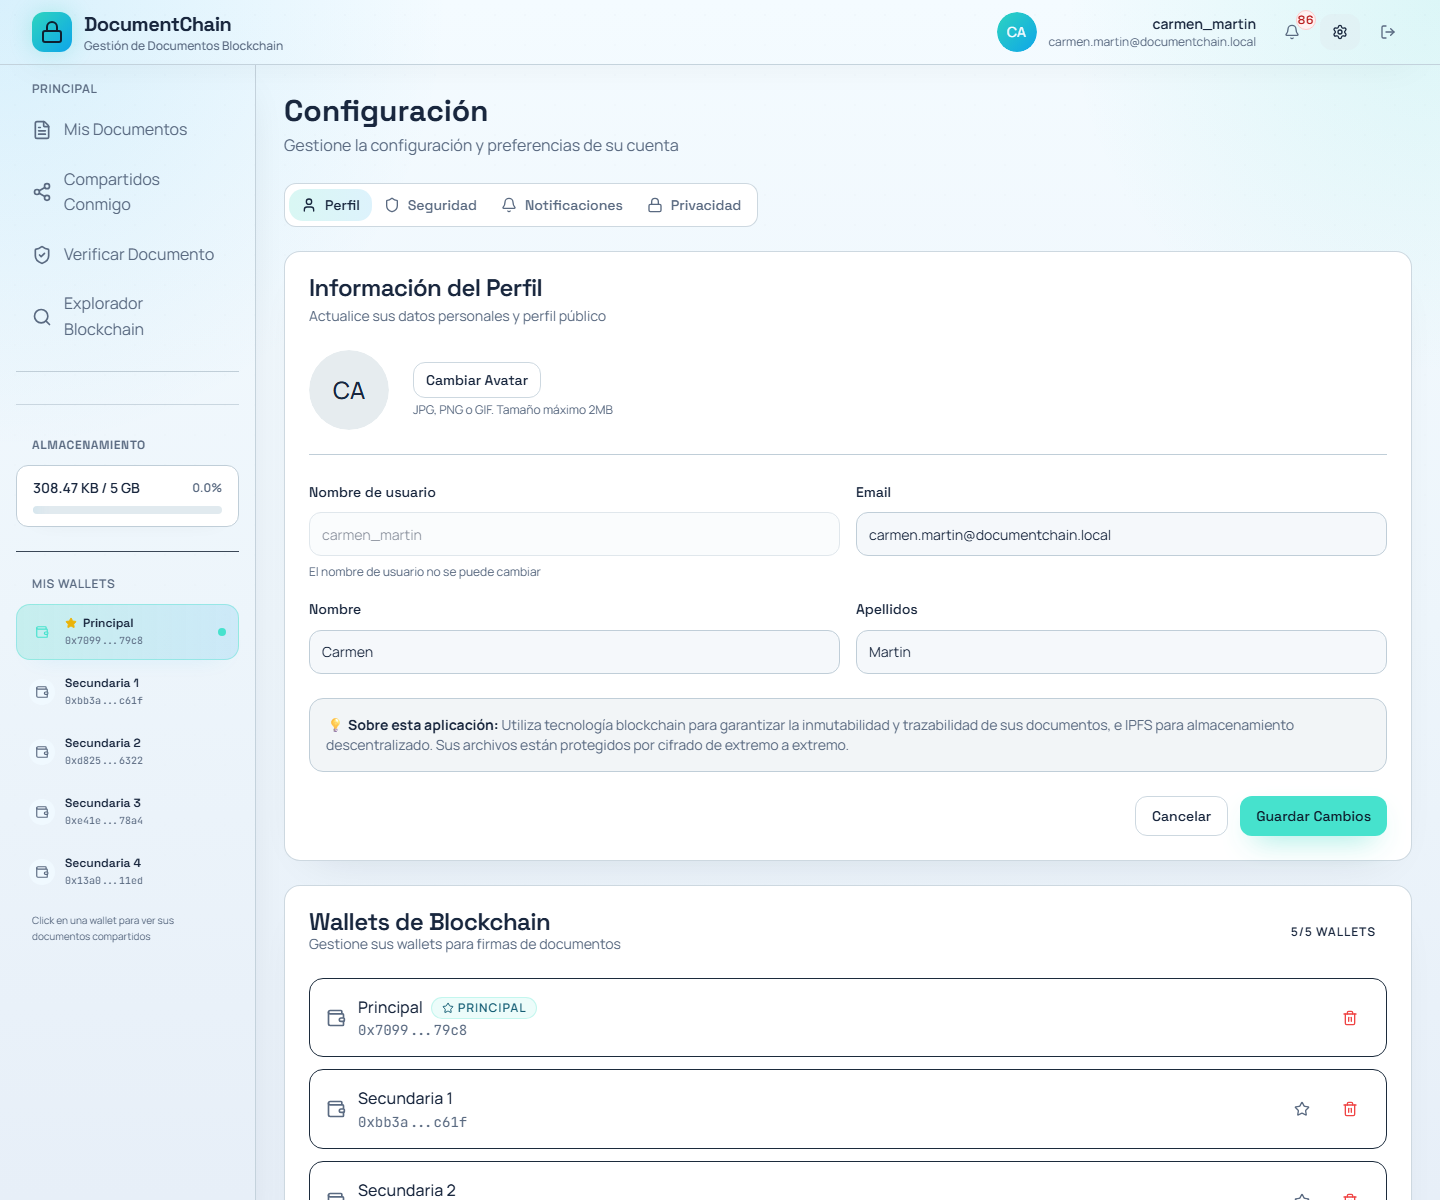
\includegraphics[width=0.45\textwidth]{capturas-ui/settings-page.png}
    \caption{Prototipo HTML (izquierda) e interfaz final (derecha) de la pagina de configuracion}
    \label{fig:mockup-settings}
\end{figure}

\subsection{Mockups de interfaz}

\begin{figure}[H]
    \centering
    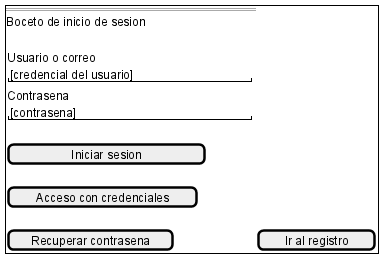
\includegraphics[width=0.8\textwidth]{diagramas/ui-login.png}
    \caption{Mockup - Pagina de inicio de sesion}
    \label{fig:ui-login}
\end{figure}

\begin{figure}[H]
    \centering
    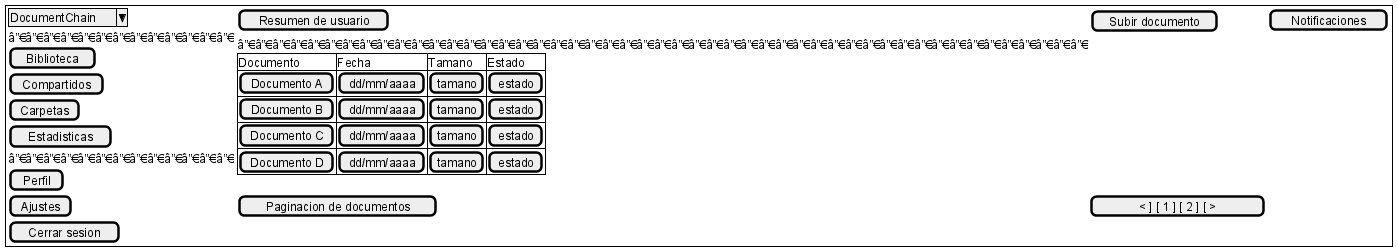
\includegraphics[width=0.8\textwidth]{diagramas/ui-dashboard.png}
    \caption{Mockup - Panel principal (biblioteca)}
    \label{fig:ui-dashboard}
\end{figure}

\begin{figure}[H]
    \centering
    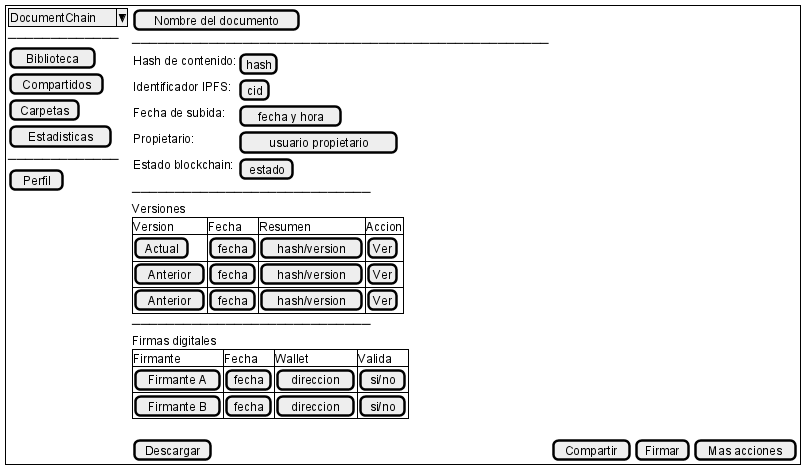
\includegraphics[width=0.8\textwidth]{diagramas/ui-document-detail.png}
    \caption{Mockup - Detalle de documento}
    \label{fig:ui-document-detail}
\end{figure}

\begin{figure}[H]
    \centering
    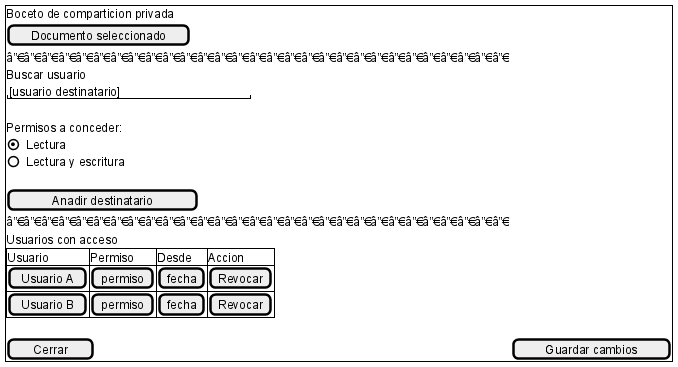
\includegraphics[width=0.8\textwidth]{diagramas/ui-share-modal.png}
    \caption{Mockup - Modal de comparticion}
    \label{fig:ui-share-modal}
\end{figure}

\begin{figure}[H]
    \centering
    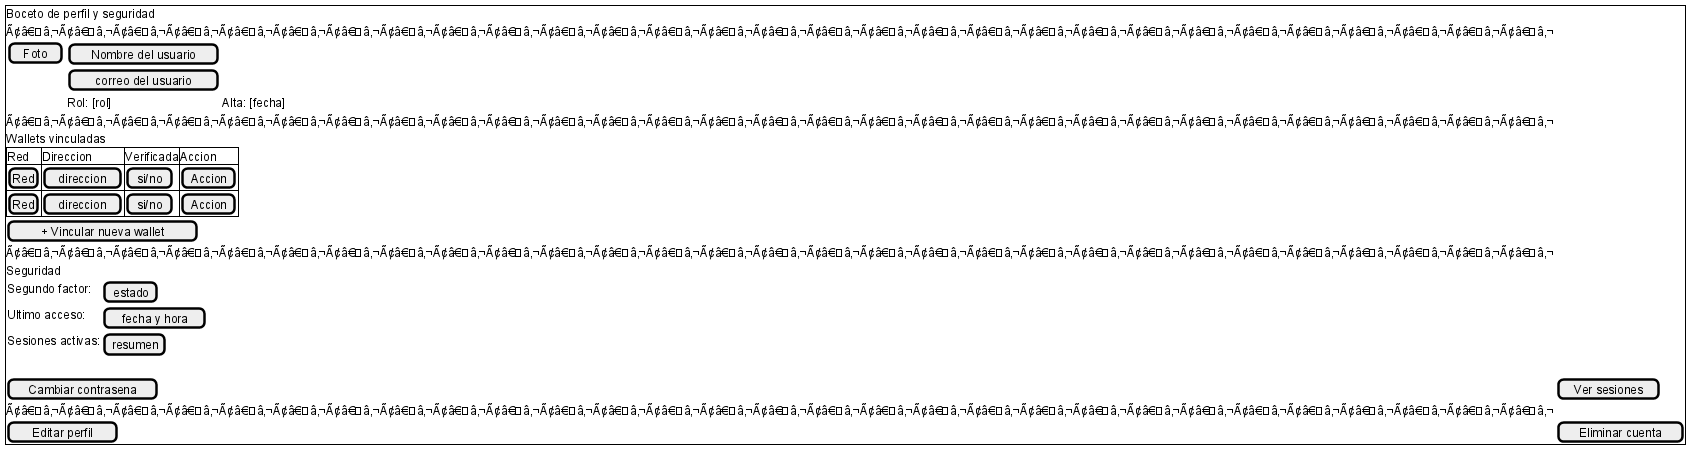
\includegraphics[width=0.8\textwidth]{diagramas/ui-profile.png}
    \caption{Mockup - Perfil de usuario}
    \label{fig:ui-profile}
\end{figure}

\begin{figure}[H]
    \centering
    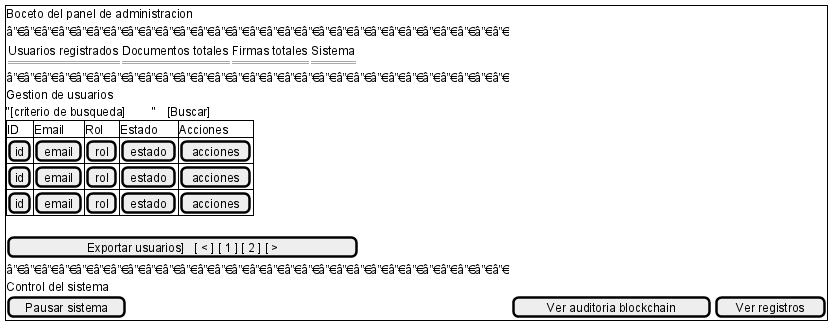
\includegraphics[width=0.8\textwidth]{diagramas/ui-admin-dashboard.png}
    \caption{Mockup - Panel de administracion}
    \label{fig:ui-admin}
\end{figure}

\section{Journey Maps}

En este apartado se documentan los mapas de viaje que capturan la experiencia del usuario en las operaciones mas representativas del sistema.

Para visualizar la experiencia completa del usuario en las operaciones mas representativas del sistema, se han elaborado mapas de viaje (\textit{journey maps}) que documentan las fases, emociones y puntos de contacto de cada flujo.

\subsection{Journey Map: Subida y firma de un documento}

\begin{table}[H]
\centering
\renewcommand{\arraystretch}{1.6}
\small
\begin{tabular}{|p{2.2cm}|p{2.8cm}|p{2.8cm}|p{2.2cm}|p{2.2cm}|}
\hline
\textbf{Fase} & \textbf{Accion del usuario} & \textbf{Respuesta del sistema} & \textbf{Emocion} & \textbf{Punto de contacto} \\
\hline
1. Descubrimiento & Abre la aplicacion e inicia sesion & Muestra el dashboard con la biblioteca de documentos & Neutra & Pagina de login \\
\hline
2. Preparacion & Selecciona ``Subir documento'' y elige archivo & Muestra modal de subida con campos de metadatos & Positiva (interfaz clara) & Modal de subida \\
\hline
3. Subida & Completa metadatos y confirma & Cifra el archivo, lo sube a IPFS y crea registro en BD & Expectante (barra de progreso) & Indicador de carga \\
\hline
4. Firma & Conecta wallet, autoriza la firma en MetaMask & Prepara transaccion para firma de wallet, verifica firma y registra en blockchain & Frustracion leve (primer uso de wallet) & Wallet externa + tutorial \\
\hline
5. Confirmacion & Espera la confirmacion on-chain & Muestra certificado de firma con txHash y enlace al explorador & Satisfaccion & Panel de detalle del documento \\
\hline
\end{tabular}
\caption{Journey map de la operacion de subida y firma documental}
\label{tab:journey-subida}
\end{table}

\textbf{Puntos de friccion identificados:} La fase de firma (paso 4) genera friccion en usuarios sin experiencia previa con wallets blockchain. La solucion implementada incluye un tutorial interactivo que se activa en el primer intento de firma y explica los conceptos de wallet, clave privada y firma digital en lenguaje accesible. Adicionalmente, la barra de progreso de la fase 3 muestra mensajes contextuales (``Cifrando archivo...'', ``Subiendo a IPFS...'', ``Preparando transaccion...'') para mantener al usuario informado durante las operaciones asincronas.

\subsection{Journey Map: Comparticion de un documento con terceros}

\begin{table}[H]
\centering
\renewcommand{\arraystretch}{1.6}
\small
\begin{tabular}{|p{2.2cm}|p{2.8cm}|p{2.8cm}|p{2.2cm}|p{2.2cm}|}
\hline
\textbf{Fase} & \textbf{Accion del usuario} & \textbf{Respuesta del sistema} & \textbf{Emocion} & \textbf{Punto de contacto} \\
\hline
1. Seleccion & Abre el detalle de un documento de su propiedad & Muestra metadatos, versiones, firmas y boton de compartir & Neutra & Pagina de detalle \\
\hline
2. Configuracion & Introduce email del destinatario y selecciona nivel de permiso & Valida que el destinatario existe en el sistema y muestra sus datos & Positiva (confirmacion visual) & Modal de comparticion \\
\hline
3. Confirmacion & Revisa los permisos y confirma & Recifra la clave simetrica para el destinatario, registra el permiso on-chain & Expectante & Wallet externa \\
\hline
4. Notificacion & Espera confirmacion & Envia email al destinatario con enlace al documento compartido & Satisfaccion & Email de notificacion \\
\hline
5. Acceso del destinatario & El destinatario accede desde ``Compartidos conmigo'' & Descifra el contenido con su clave privada y muestra el documento & Positiva (acceso inmediato) & Vista de documentos compartidos \\
\hline
\end{tabular}
\caption{Journey map de la operacion de comparticion documental}
\label{tab:journey-comparticion}
\end{table}

\textbf{Puntos de friccion identificados:} Los usuarios interpretaban inicialmente el boton ``Compartir'' como un envio del archivo por correo, no como una concesion de permisos on-chain. La interfaz se rediseno para mostrar explicitamente los tres niveles de permiso (Lector, Editor) con descripciones breves. Ademas, el email de notificacion incluye un enlace directo a la vista ``Compartidos conmigo'' dentro de la aplicacion, no al archivo en si, reforzando el modelo mental de acceso controlado.

\section{Comparativa wireframe a interfaz final}

Para ilustrar la evolucion del diseno desde la fase de prototipado hasta la implementacion final, se presentan a continuacion comparativas lado a lado de las pantallas principales del sistema. Los wireframes (izquierda) corresponden a los prototipos de baja fidelidad generados con PlantUML durante la fase de analisis. Las capturas de la interfaz final (derecha) muestran el resultado de la implementacion en React con Tailwind CSS y componentes shadcn/ui.

\begin{figure}[H]
    \centering
    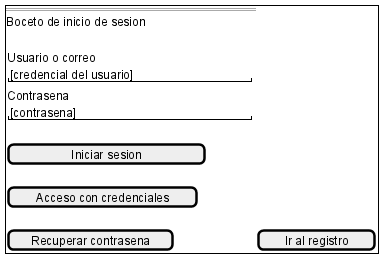
\includegraphics[width=0.45\textwidth]{diagramas/ui-login.png}\hfill
    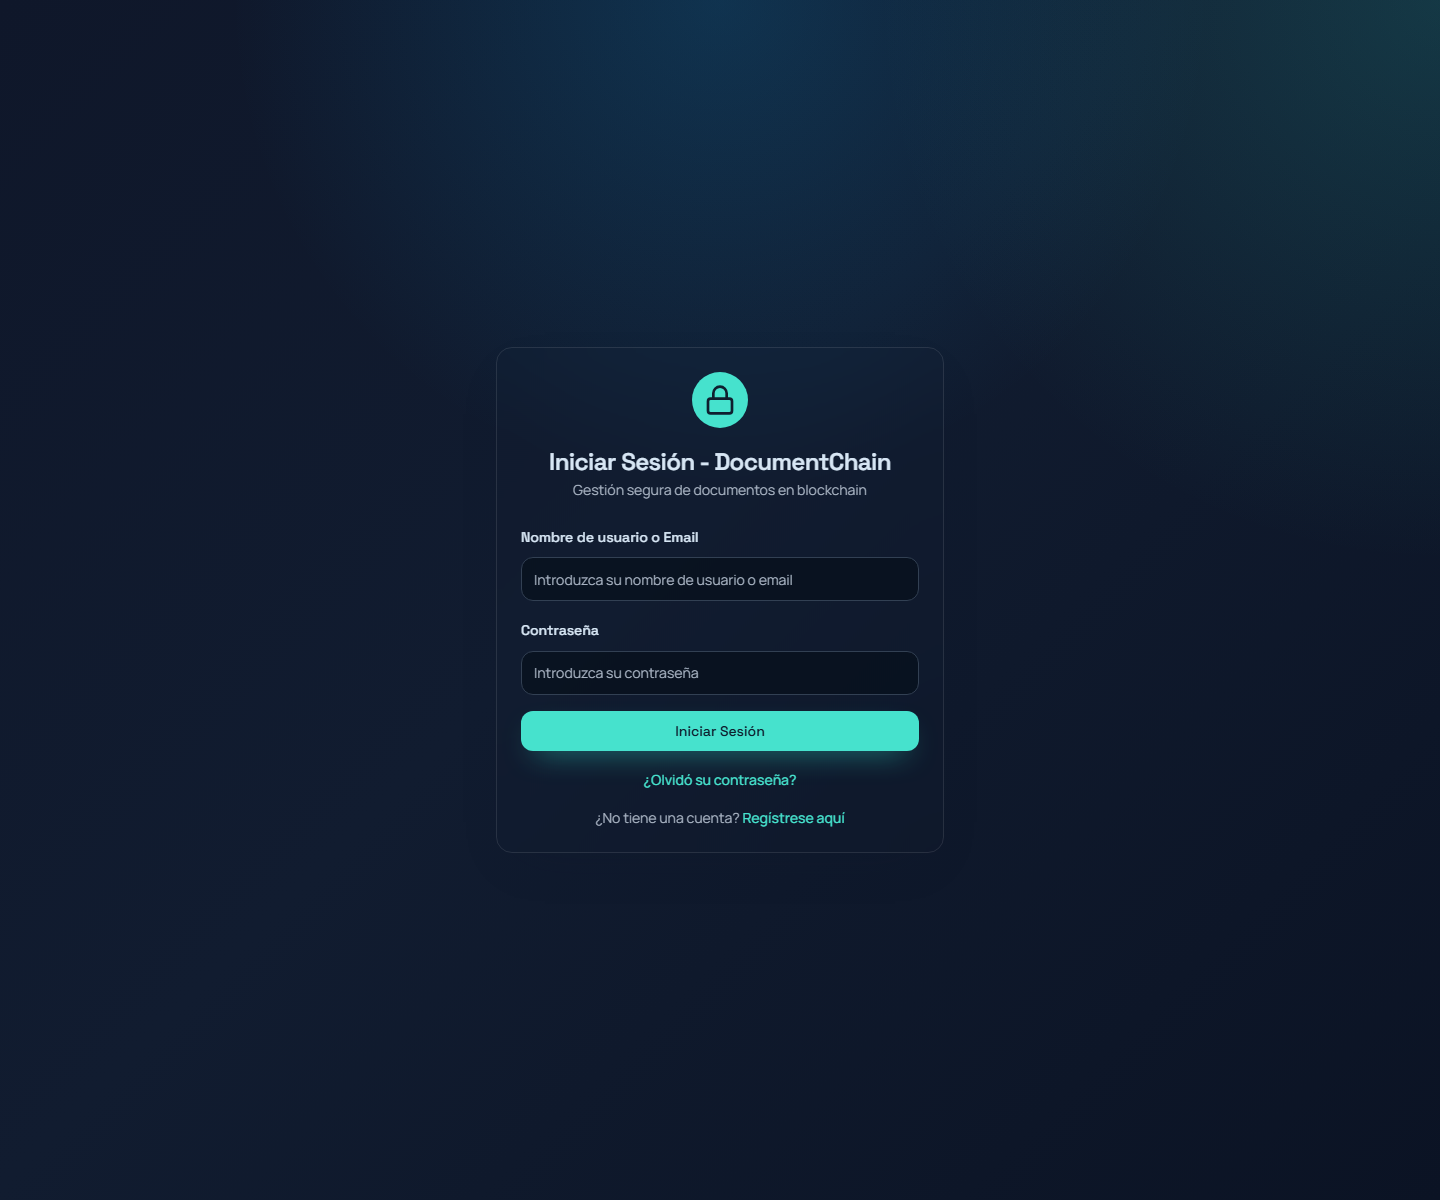
\includegraphics[width=0.45\textwidth]{capturas-ui/login-page.png}
    \caption{Comparativa: wireframe de inicio de sesion (izquierda) vs. implementacion final (derecha)}
    \label{fig:cmp-login}
\end{figure}

\begin{figure}[H]
    \centering
    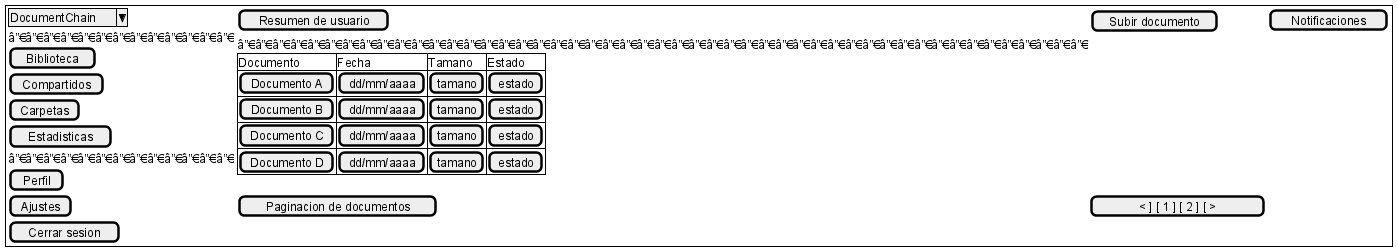
\includegraphics[width=0.45\textwidth]{diagramas/ui-dashboard.png}\hfill
    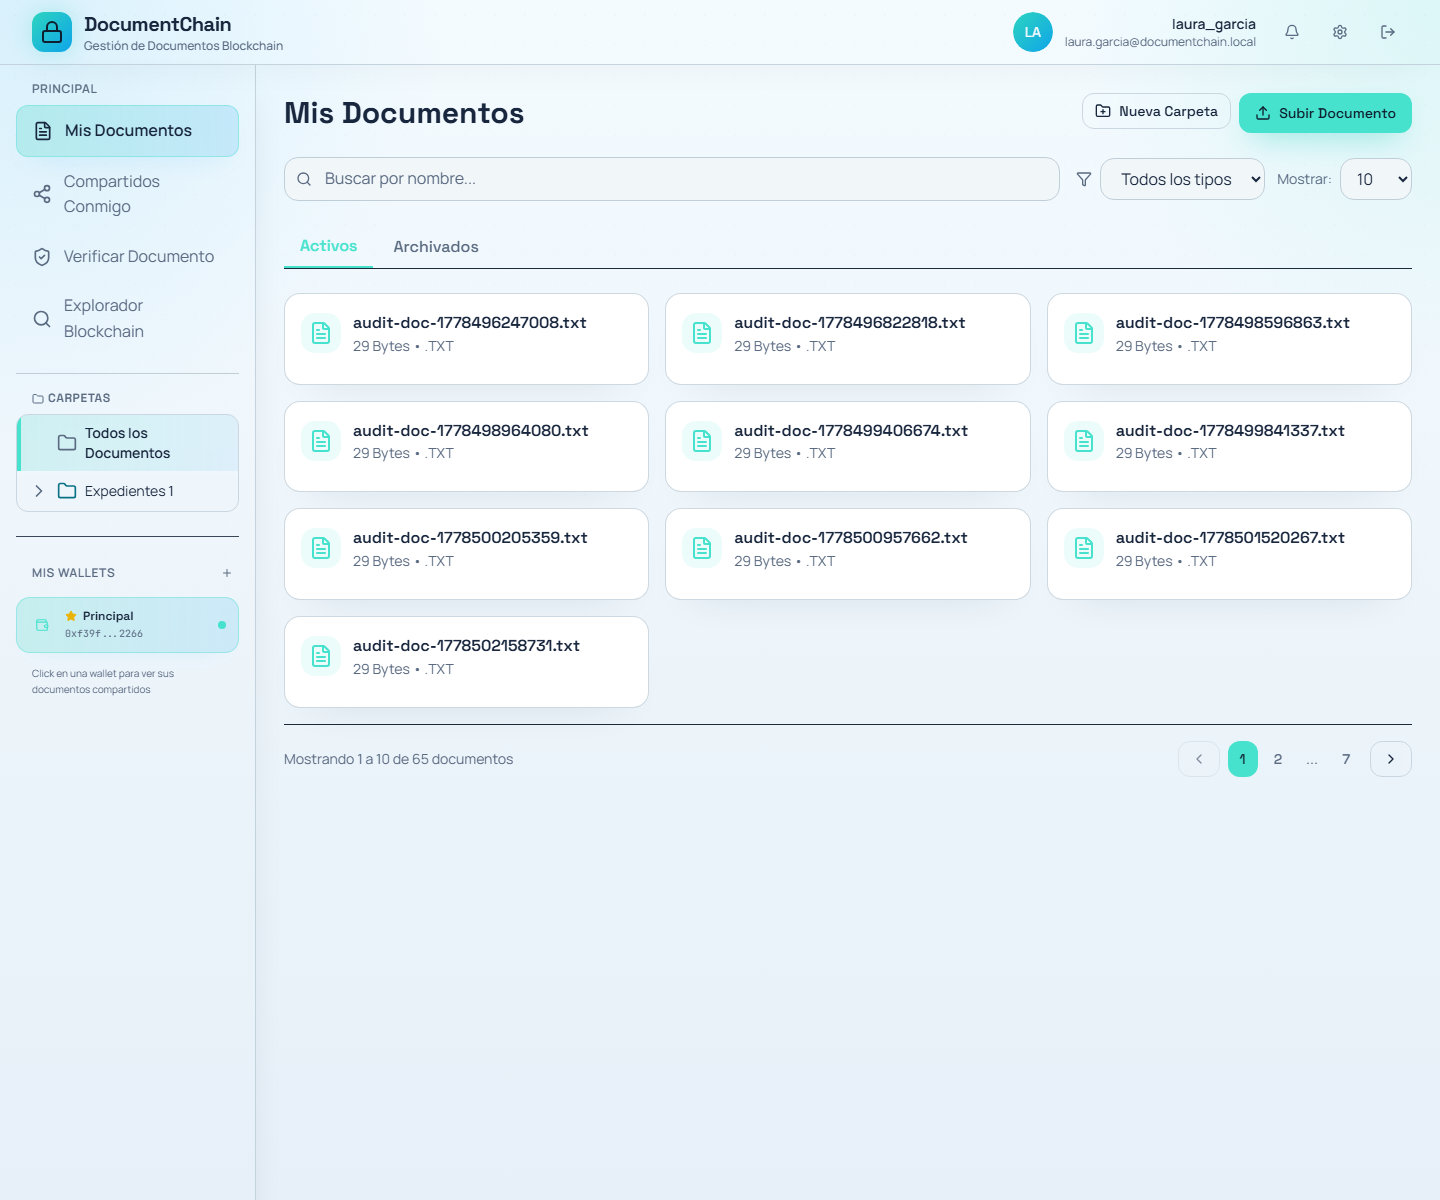
\includegraphics[width=0.45\textwidth]{capturas-ui/documents-page.png}
    \caption{Comparativa: wireframe de biblioteca (izquierda) vs. implementacion final (derecha)}
    \label{fig:cmp-dashboard}
\end{figure}

\begin{figure}[H]
    \centering
    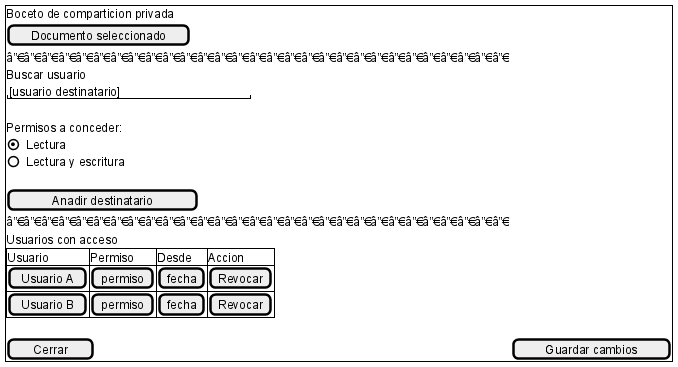
\includegraphics[width=0.45\textwidth]{diagramas/ui-share-modal.png}\hfill
    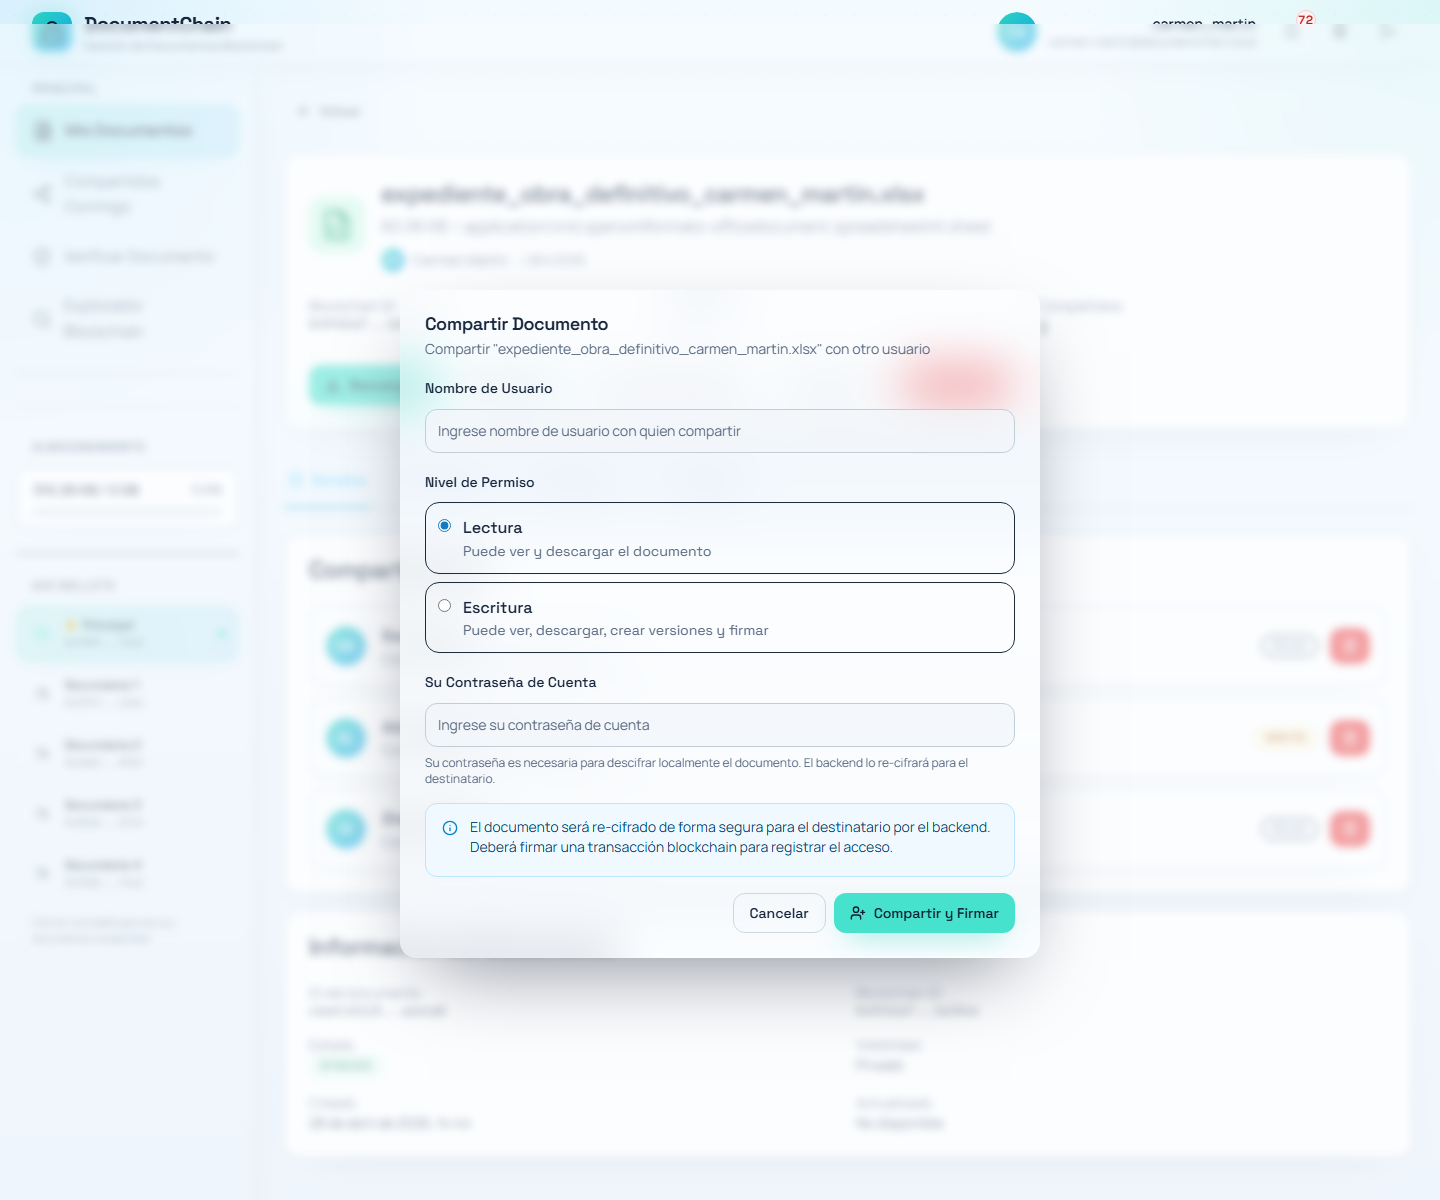
\includegraphics[width=0.45\textwidth]{capturas-ui/share-modal.png}
    \caption{Comparativa: wireframe de comparticion (izquierda) vs. implementacion final (derecha)}
    \label{fig:cmp-share}
\end{figure}

\begin{figure}[H]
    \centering
    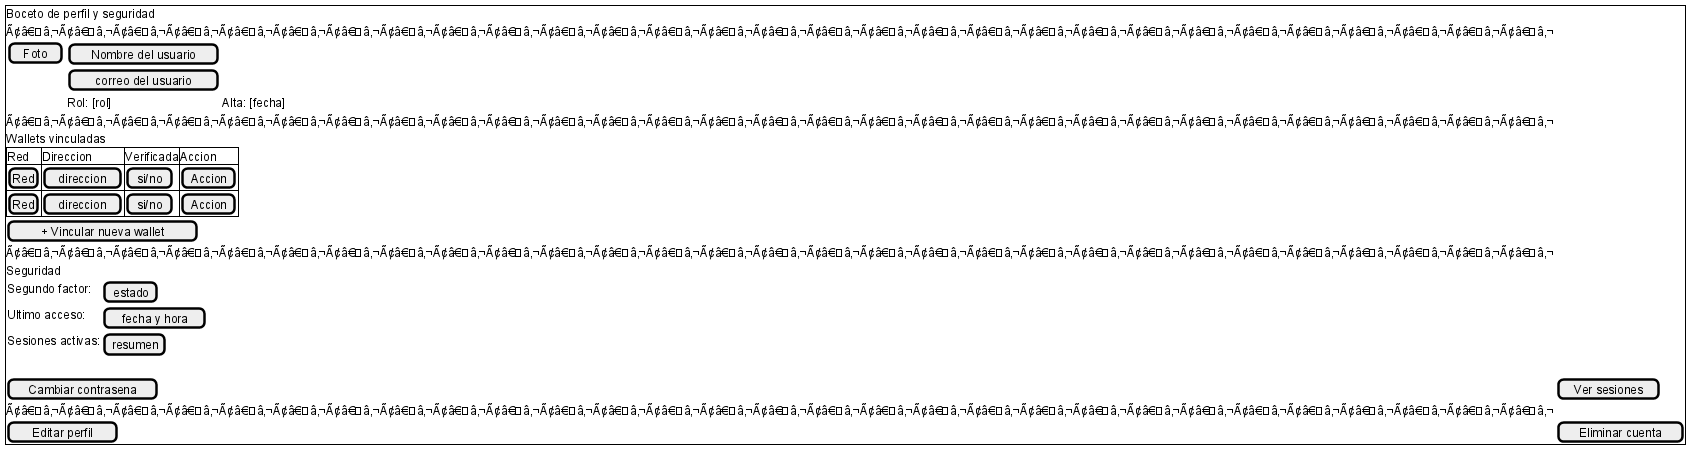
\includegraphics[width=0.45\textwidth]{diagramas/ui-profile.png}\hfill
    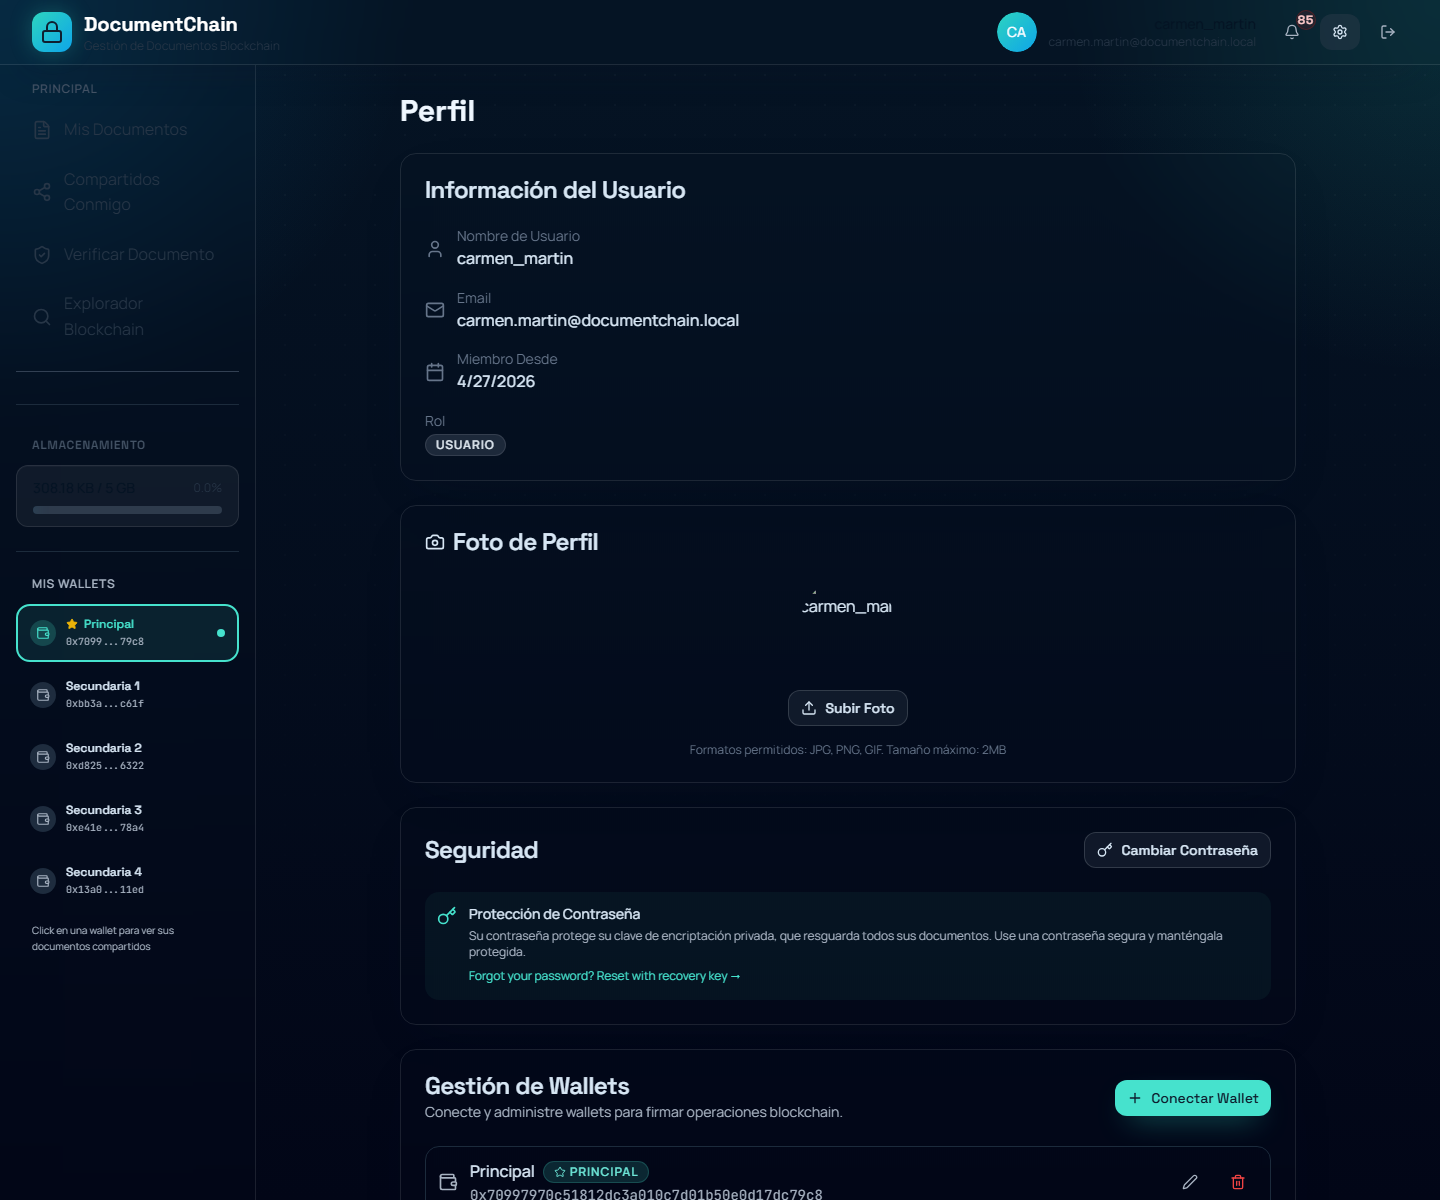
\includegraphics[width=0.45\textwidth]{capturas-ui/profile-page.png}
    \caption{Comparativa: wireframe de perfil (izquierda) vs. implementacion final (derecha)}
    \label{fig:cmp-profile}
\end{figure}

\begin{figure}[H]
    \centering
    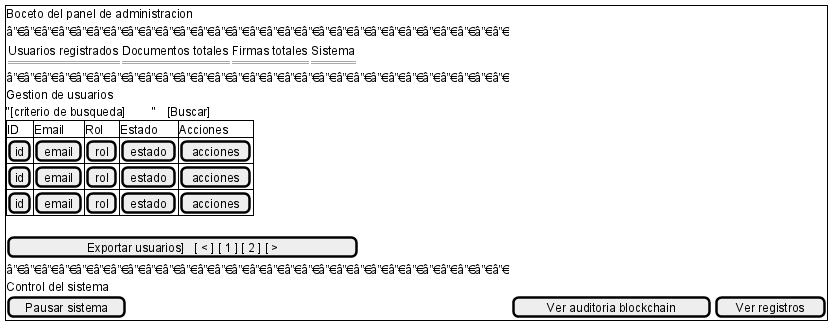
\includegraphics[width=0.45\textwidth]{diagramas/ui-admin-dashboard.png}\hfill
    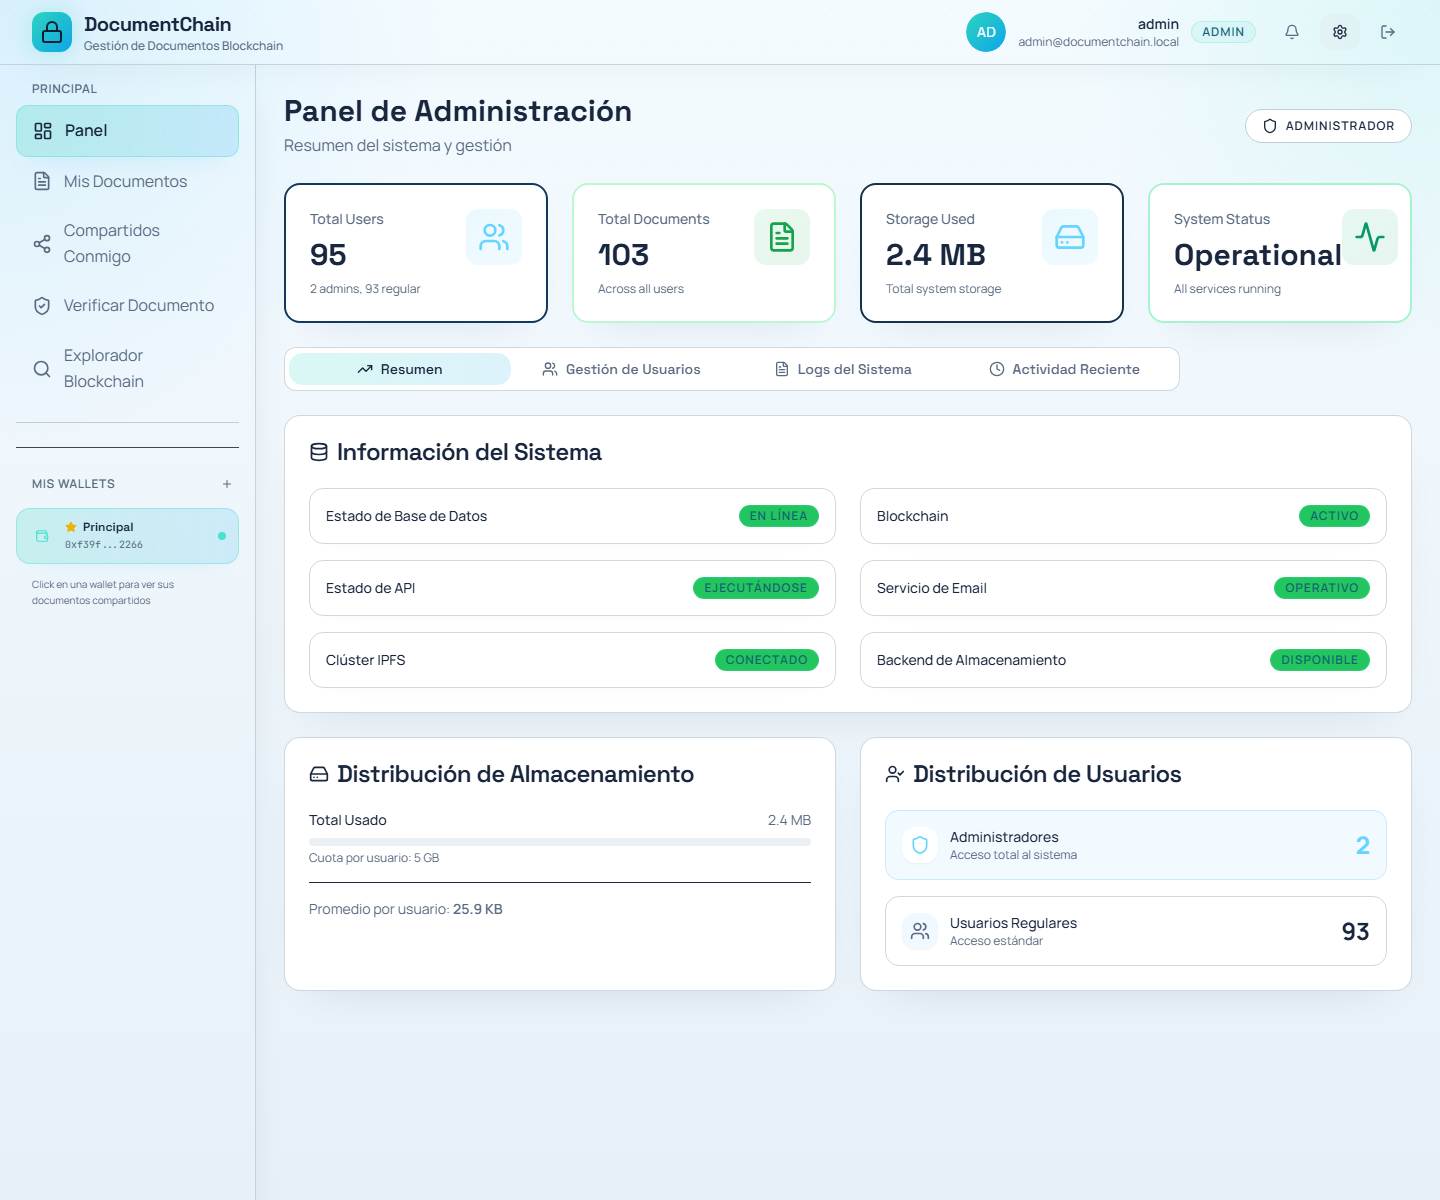
\includegraphics[width=0.45\textwidth]{capturas-ui/admin-dashboard.png}
    \caption{Comparativa: wireframe de administracion (izquierda) vs. implementacion final (derecha)}
    \label{fig:cmp-admin}
\end{figure}

Las comparativas evidencian una alta fidelidad entre los prototipos iniciales y la implementaci\'on final. Esto indica que el proceso de dise\~no centrado en el usuario fue efectivo a la hora de traducir los requisitos de usabilidad a componentes funcionales. Las diferencias que se aprecian corresponden sobre todo a refinamientos visuales propios de la implementaci\'on: paleta de colores corporativa, tipograf\'ia del sistema y espaciado responsive. Tambi\'en se incorporaron elementos que surgieron durante las pruebas de usabilidad, como el tutorial interactivo de wallet, los indicadores de progreso y los di\'alogos de confirmaci\'on contextuales.

\section{Principios de diseno aplicados}

En este apartado se exponen los principios heuristicos que fundamentan el diseno de la interfaz de DocumentChain.

El diseno de la interfaz de DocumentChain se fundamenta en los siguientes principios, extraidos de las heuristicas de usabilidad de Nielsen y adaptados al contexto de una aplicacion descentralizada:

\begin{enumerate}
    \item \textbf{Visibilidad del estado del sistema.} Cada operacion blockchain muestra su estado actual mediante indicadores visuales y textuales: ``Preparando...'', ``Pendiente de firma...'', ``Confirmando en blockchain...'', ``Sincronizado''. El usuario siempre sabe en que punto del flujo se encuentra.
    \item \textbf{Correspondencia con el mundo real.} La terminologia evita tecnicismos innecesarios. En lugar de ``transmitir transaccion a la red'', se utiliza ``registrando en blockchain''. El concepto de ``firma digital'' se explica mediante una analogia con la firma manuscrita tradicional.
    \item \textbf{Control y libertad del usuario.} Las operaciones criticas (eliminacion de cuenta, transferencia de propiedad, revocacion de acceso) requieren confirmacion explicita e incluyen una opcion de cancelacion en cada paso. Las transacciones blockchain no se envian hasta que el usuario las firma explicitamente en su wallet.
    \item \textbf{Consistencia y estandares.} La interfaz mantiene una estructura de navegacion consistente: barra lateral con las secciones principales, area de contenido central con breadcrumbs, y barra superior con notificaciones y perfil. Los componentes shadcn/ui garantizan coherencia visual en todos los dialogos, tablas y formularios.
    \item \textbf{Prevencion de errores.} Los campos de entrada incluyen validacion en tiempo real. Las operaciones sobre documentos archivados se deshabilitan con un mensaje explicativo. La conexion de wallets invalidas se rechaza antes de iniciar cualquier flujo.
    \item \textbf{Flexibilidad y eficiencia.} Los usuarios avanzados pueden utilizar atajos de teclado y la API REST directamente. La interfaz ofrece tanto una vista simplificada para usuarios noveles como acceso a metadatos tecnicos (hash de transaccion, direccion del contrato, numero de bloque) para usuarios expertos.
\end{enumerate}

\subsection{Storyboard 1: Subida y firma de contrato}

\begin{enumerate}
    \item El usuario abre la aplicacion e inicia sesion.
    \item Navega a la biblioteca y selecciona ``Subir documento''.
    \item Carga el archivo PDF del contrato y completa los metadatos.
    \item Conecta su wallet de MetaMask.
    \item Selecciona ``Firmar documento'' y confirma la transaccion.
    \item El sistema muestra el certificado de firma con el hash en blockchain.
\end{enumerate}

\subsection{Storyboard 2: Verificacion publica por tercero}

\begin{enumerate}
    \item Un tercero recibe un enlace de verificacion por email.
    \item Accede a la pagina publica sin necesidad de cuenta.
    \item Escanea el codigo QR o introduce el ID publico.
    \item El sistema muestra el estado de verificacion, propietario y firmas.
    \item El tercero verifica que el documento es autentico y no ha sido modificado.
\end{enumerate}

\section{Pruebas de usabilidad}

En este apartado se documentan las pruebas de usabilidad realizadas sobre el sistema, incluyendo la metodologia, los resultados y las iteraciones de mejora derivadas de los hallazgos.

\subsection{Metodologia}

En este apartado se describe la metodologia seguida para evaluar la usabilidad del sistema.

Las pruebas de usabilidad se disenaron siguiendo una metodologia mixta que combina evaluacion cuantitativa mediante el cuestionario \textbf{System Usability Scale (SUS)} de Brooke (1996) y observacion cualitativa mediante el protocolo \textit{think-aloud}. Se reclutaron 5 participantes de perfil no tecnico con edades comprendidas entre 22 y 45 anos, ninguno de los cuales tenia experiencia previa con wallets blockchain ni con IPFS.

Cada sesion tuvo una duracion de aproximadamente 45 minutos y se estructuro en tres fases:

\begin{enumerate}
    \item \textbf{Onboarding guiado} (10 min): presentacion del sistema, creacion de cuenta y verificacion de email, sin asistencia del evaluador.
    \item \textbf{Tareas guiadas} (25 min): ejecucion de 6 tareas predefinidas mientras el participante verbalizaba sus pensamientos (protocolo \textit{think-aloud}):
    \begin{enumerate}
        \item Subir un documento y verificar su registro en la lista.
        \item Compartir el documento con otro usuario otorgando permisos de solo lectura.
        \item Firmar digitalmente el documento mediante una wallet conectada.
        \item Verificar la autenticidad del documento desde la pagina publica (sin iniciar sesion).
        \item Crear una nueva version del documento y establecerla como operativa.
        \item Transferir la propiedad del documento a otro usuario.
    \end{enumerate}
    \item \textbf{Cuestionario SUS y entrevista} (10 min): cumplimentacion del cuestionario estandarizado de 10 items y entrevista semi-estructurada para recoger impresiones generales.
\end{enumerate}

\subsection{Resultados cuantitativos}

La Tabla~\ref{tab:sus} recoge las puntuaciones SUS obtenidas por cada participante.

\begin{table}[H]
\centering
\renewcommand{\arraystretch}{1.3}
\begin{tabular}{|c|c|c|}
\hline
\textbf{Participante} & \textbf{Perfil} & \textbf{Puntuacion SUS} \\
\hline
P1 & Profesional juridico & 72 \\
\hline
P2 & Profesional juridico & 68 \\
\hline
P3 & Administrativo & 74 \\
\hline
P4 & Estudiante de grado & 81 \\
\hline
P5 & Estudiante de grado & 78 \\
\hline
\textbf{Media} & & \textbf{74,6} \\
\hline
\end{tabular}
\caption{Puntuaciones SUS por participante}
\label{tab:sus}
\end{table}

La puntuacion media de 74,6 se situa en el rango \textit{good} (68--80) segun la escala de adjetivos de Bangor, Kortum y Miller (2009), y por encima del percentil 68 de la distribucion de referencia. Este resultado indica que el sistema es percibido como usable por usuarios sin experiencia previa en blockchain, aunque existe margen de mejora para alcanzar el umbral \textit{excellent} (por encima de 80).

\subsection{Hallazgos cualitativos}

El analisis de las sesiones \textit{think-aloud} revelo los siguientes patrones recurrentes:

\begin{itemize}
    \item \textbf{Conexion de wallet}. Fue el punto mas critico para los 5 participantes. Tres de ellos no comprendian el concepto de wallet como identidad blockchain independiente de la cuenta de la plataforma. Como resultado, se incorporo un tutorial interactivo que aparece en el primer intento de firma, explicando en lenguaje no tecnico la relacion entre la cuenta de usuario y la wallet Ethereum.
    \item \textbf{Modal de comparticion}. Cuatro participantes interpretaron inicialmente el boton ``Compartir'' como un envio del archivo por correo electronico, no como una concesion de permisos on-chain. Se rediseno el modal para mostrar explicitamente los tres niveles de permiso (Lector, Editor, Propietario) con descripciones breves en lugar de iconos ambiguos.
    \item \textbf{Terminologia}. Los terminos ``archivar'' y ``eliminar'' generaron confusion en 3 participantes, que los percibian como sinonimos. Se anadio un dialogo de confirmacion que explica la diferencia: archivar oculta el documento de la lista pero preserva su integridad y permisos, mientras que eliminar es una operacion irreversible.
    \item \textbf{Verificacion publica}. Cuatro participantes valoraron muy positivamente la pagina de verificacion publica, destacando su simplicidad (un unico campo de texto) frente a la complejidad del resto de la interfaz. Este hallazgo reforzo la decision de diseno de mantener la verificacion publica como un flujo radicalmente simplificado, accesible sin registro previo.
    \item \textbf{Tiempos de respuesta}. Dos participantes manifestaron inquietud durante la espera de confirmacion de transacciones blockchain (estado ``Preparando...''). Se anadio un indicador de progreso estimado y un aviso que explica que la operacion esta siendo registrada en la blockchain para garantizar su inmutabilidad.
\end{itemize}

\subsection{Iteraciones de diseno}

Con base en los hallazgos descritos, se realizaron las siguientes iteraciones:

\begin{itemize}
    \item \textbf{Iteracion 1}: Incorporacion del tutorial interactivo de wallet, rediseno del modal de comparticion con etiquetas textuales de permisos y dialogo de confirmacion para operaciones de archivado.
    \item \textbf{Iteracion 2} (validacion): Dos de los participantes originales (P3 y P5) repitieron las tareas 2, 3 y 4 sobre la version modificada. Los tiempos de ejecucion se redujeron en un 35\% en promedio, y la puntuacion SUS de la segunda pasada ascendio a 82 (P3) y 86 (P5), sugiriendo que las modificaciones abordaron eficazmente los puntos de friccion identificados.
\end{itemize}

Estas pruebas, aunque con un tamano muestral reducido, proporcionaron evidencia suficiente para orientar el diseno de la interfaz hacia un equilibrio entre la complejidad tecnica del dominio blockchain y la usabilidad esperable por un publico general.

\end{document}



